\documentclass{article}\usepackage[]{graphicx}\usepackage[]{color}
%% maxwidth is the original width if it is less than linewidth
%% otherwise use linewidth (to make sure the graphics do not exceed the margin)
\makeatletter
\def\maxwidth{ %
  \ifdim\Gin@nat@width>\linewidth
    \linewidth
  \else
    \Gin@nat@width
  \fi
}
\makeatother

\definecolor{fgcolor}{rgb}{0.345, 0.345, 0.345}
\newcommand{\hlnum}[1]{\textcolor[rgb]{0.686,0.059,0.569}{#1}}%
\newcommand{\hlstr}[1]{\textcolor[rgb]{0.192,0.494,0.8}{#1}}%
\newcommand{\hlcom}[1]{\textcolor[rgb]{0.678,0.584,0.686}{\textit{#1}}}%
\newcommand{\hlopt}[1]{\textcolor[rgb]{0,0,0}{#1}}%
\newcommand{\hlstd}[1]{\textcolor[rgb]{0.345,0.345,0.345}{#1}}%
\newcommand{\hlkwa}[1]{\textcolor[rgb]{0.161,0.373,0.58}{\textbf{#1}}}%
\newcommand{\hlkwb}[1]{\textcolor[rgb]{0.69,0.353,0.396}{#1}}%
\newcommand{\hlkwc}[1]{\textcolor[rgb]{0.333,0.667,0.333}{#1}}%
\newcommand{\hlkwd}[1]{\textcolor[rgb]{0.737,0.353,0.396}{\textbf{#1}}}%

\usepackage{framed}
\makeatletter
\newenvironment{kframe}{%
 \def\at@end@of@kframe{}%
 \ifinner\ifhmode%
  \def\at@end@of@kframe{\end{minipage}}%
  \begin{minipage}{\columnwidth}%
 \fi\fi%
 \def\FrameCommand##1{\hskip\@totalleftmargin \hskip-\fboxsep
 \colorbox{shadecolor}{##1}\hskip-\fboxsep
     % There is no \\@totalrightmargin, so:
     \hskip-\linewidth \hskip-\@totalleftmargin \hskip\columnwidth}%
 \MakeFramed {\advance\hsize-\width
   \@totalleftmargin\z@ \linewidth\hsize
   \@setminipage}}%
 {\par\unskip\endMakeFramed%
 \at@end@of@kframe}
\makeatother

\definecolor{shadecolor}{rgb}{.97, .97, .97}
\definecolor{messagecolor}{rgb}{0, 0, 0}
\definecolor{warningcolor}{rgb}{1, 0, 1}
\definecolor{errorcolor}{rgb}{1, 0, 0}
\newenvironment{knitrout}{}{} % an empty environment to be redefined in TeX

\usepackage{alltt}
\usepackage[T1]{fontenc}
\usepackage[utf8]{inputenc}

\usepackage{amsmath}
\usepackage{graphicx}
%\usepackage{bbold}
\usepackage{tikz}
%\usepackage{silence}
\usepackage{mdframed}

%\WarningFilter{mdframed}{You got a bad break}
\usepackage[colorinlistoftodos]{todonotes}
\usepackage{listings}
%\usepackage{listingsutf8}
\usepackage{color}
\colorlet{exampcol}{blue!10}
\usepackage{multicol}
\usepackage[answerdelayed]{exercise}
\title{BIO311: Population Ecology\\ \textit{Practical 7 (Unstructured populations)}}


%\author{Timoth\'ee Bonnet \& Koen van Benthem\\\\
%\tt{timothee.bonnet@ieu.uzh.ch}\\ \tt{koen.vanbenthem@ieu.uzh.ch}}

%\date{Spring 2016}
\setcounter{tocdepth}{1} % Determines the depth of the table of contents;; 0:chapters, 1: chapters and sections, 2: chapters,sections and subsections

%\renewcommand{\theExercise}{\thechapter.\arabic{Exercise}}%
\setlength\parindent{0pt}
\IfFileExists{upquote.sty}{\usepackage{upquote}}{}
\begin{document}

\author{Timoth\'ee Bonnet \&\footnote{This document was co-authored by Tina Cornioley}\; Koen van Benthem\\\\
\tt{timothee.bonnet@ieu.uzh.ch}\\ \tt{koen.vanbenthem@ieu.uzh.ch}}

\date{Spring 2016}


\maketitle
\tableofcontents


\newpage


\section{Discrete Population Growth}
The botanical garden created a new pond in $2009$ and introduced one plant of pond-lily. This population produces offspring each spring and grows with a discrete growth factor $\lambda$ of $3$, $N_t=N_0\lambda ^t$ : after the first year, there were three individuals; $3=1 \cdot (3)^1$, by the second year the botanical garden had six more and in 2013, the total population size was $81$.

\vspace{1.5ex}

\begin{center}
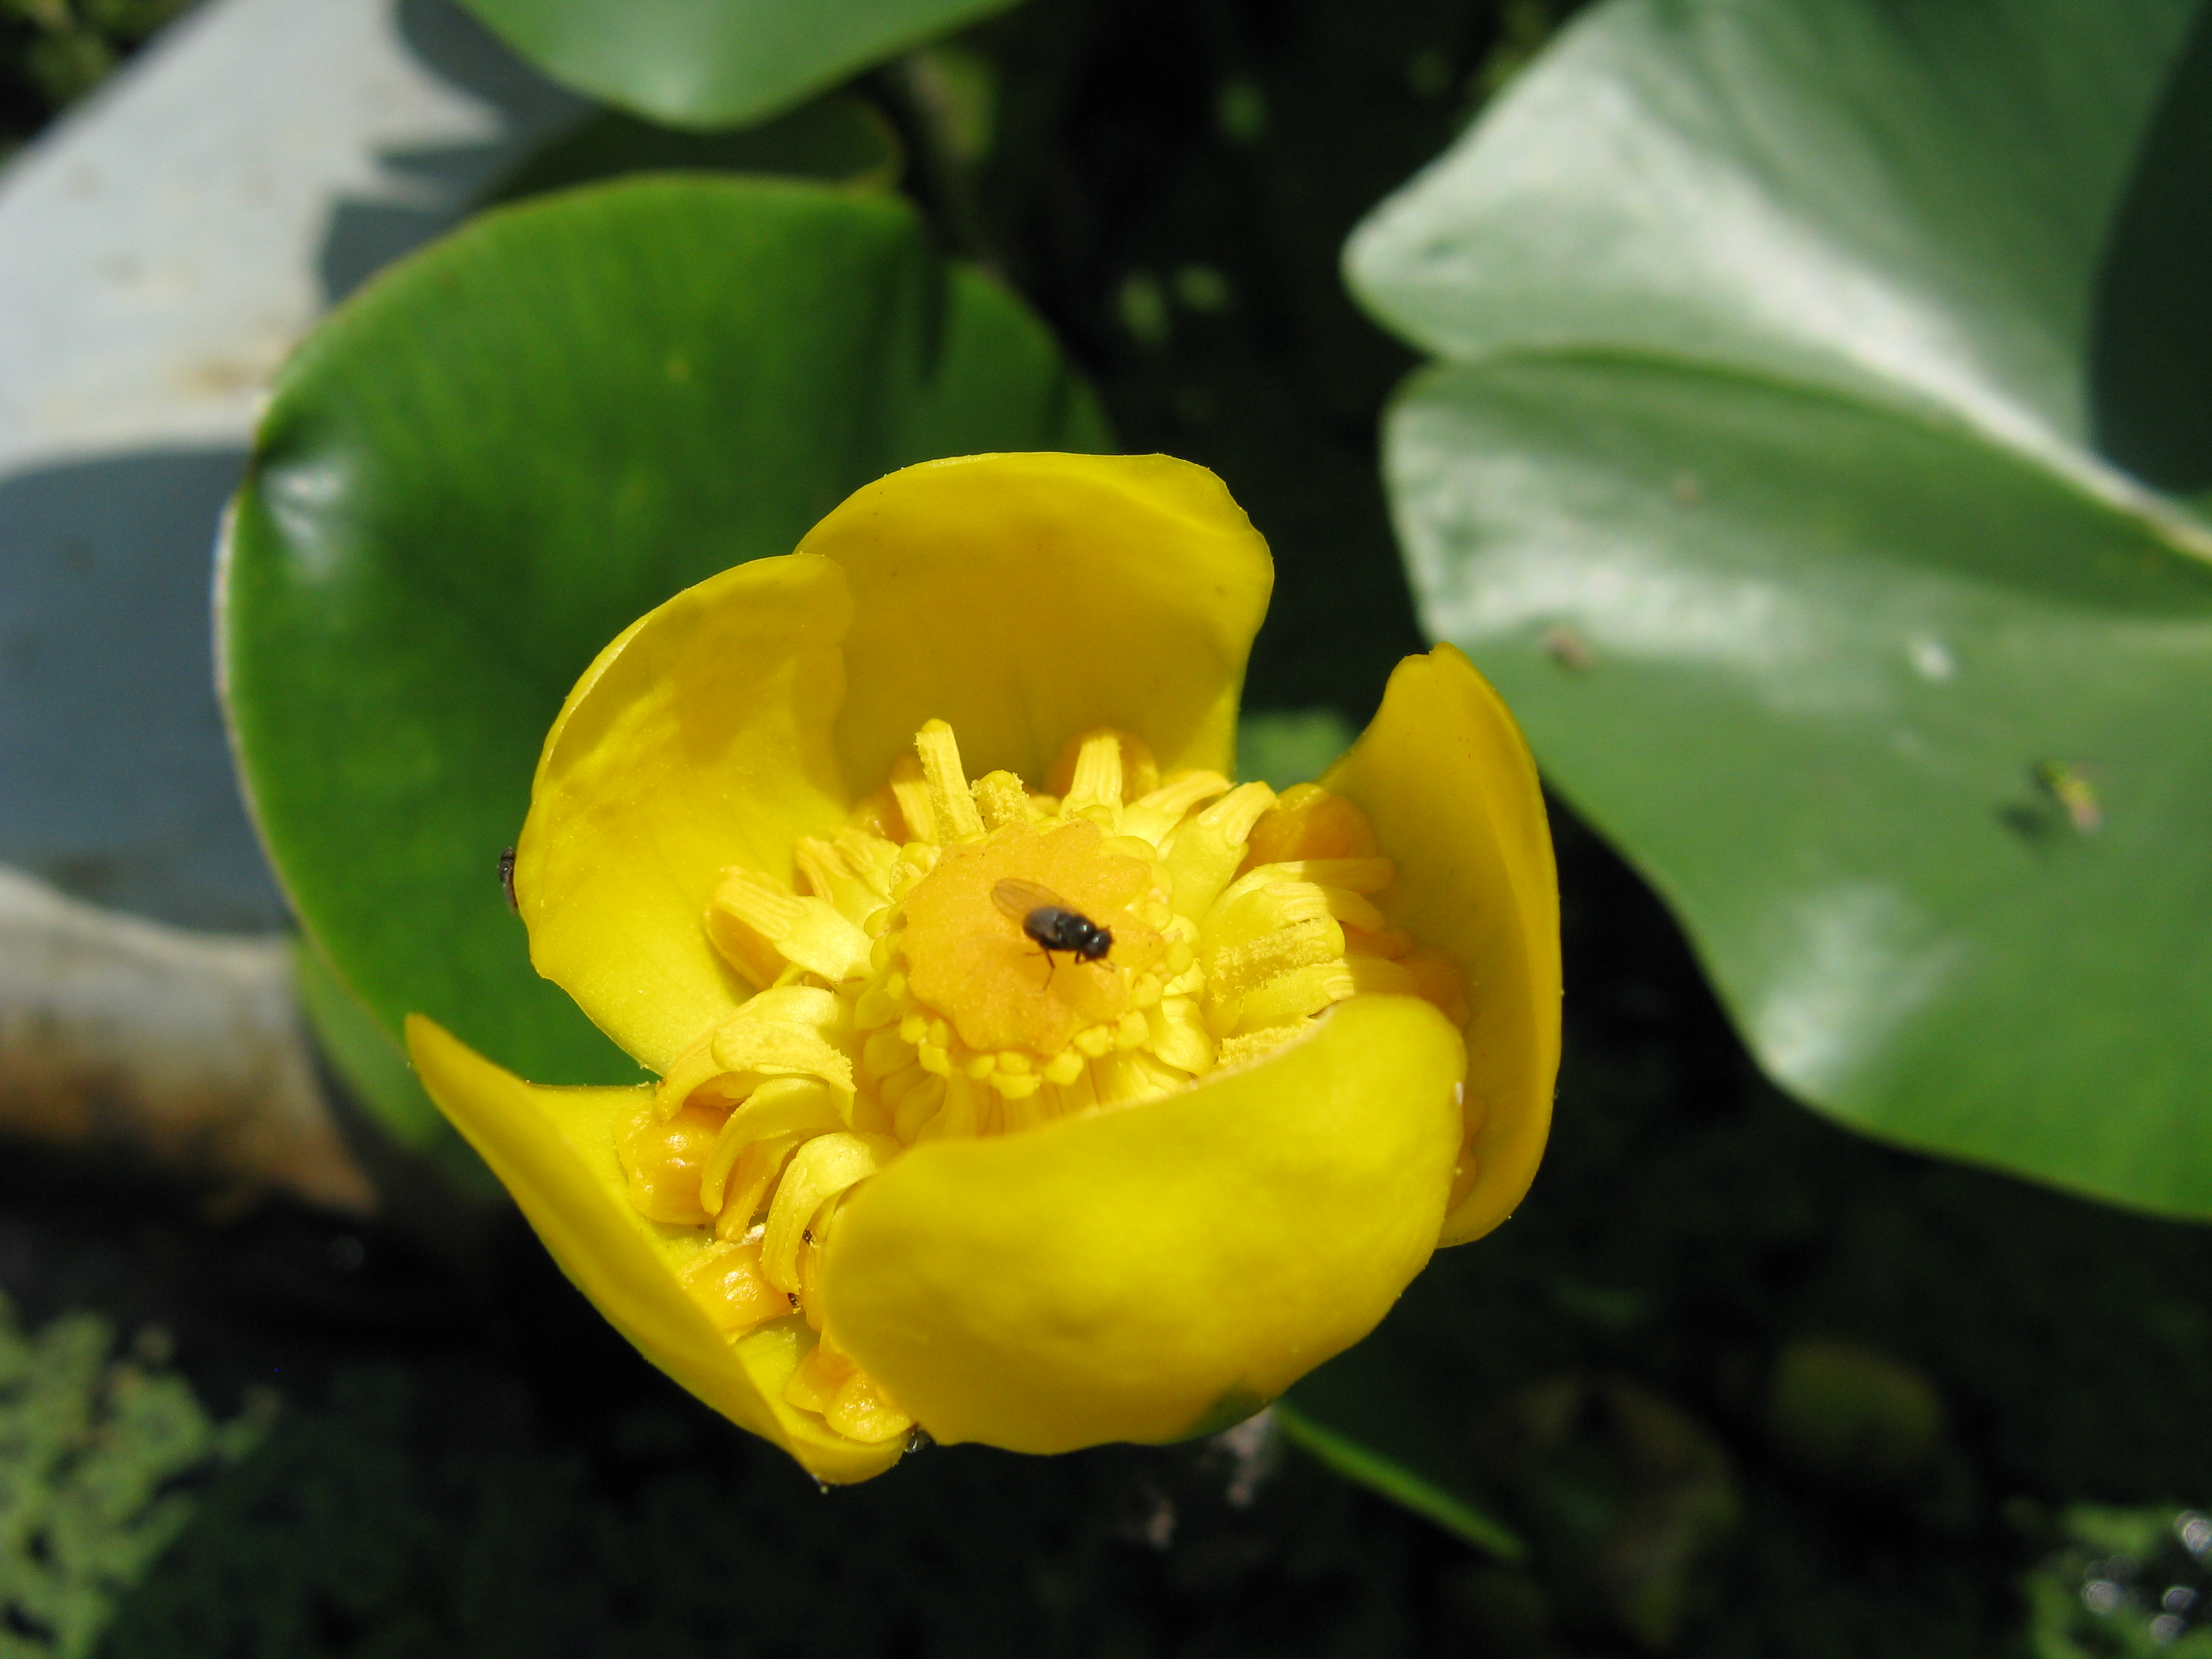
\includegraphics[width=0.65\textwidth]{Nuphar_pumilum2.jpg}
\end{center}
\vspace{1.5ex}

Let us look at the evolution of population size over time. First we define the values of our different parameters.
\begin{knitrout}
\definecolor{shadecolor}{rgb}{0.969, 0.969, 0.969}\color{fgcolor}\begin{kframe}
\begin{alltt}
\hlstd{N0} \hlkwb{<-} \hlnum{1}
\hlstd{lambda} \hlkwb{<-} \hlnum{3}
\hlstd{t} \hlkwb{<-} \hlnum{0}\hlopt{:}\hlnum{4}
\end{alltt}
\end{kframe}
\end{knitrout}
Now, we get the population size over time and we plot this in a graph. The code \texttt{axis} sets the label below the x-axis to be $2009$, $2010$, $2011$, $2012$, $2013$. The \textasciicircum  \; sign means \textquotedblleft raise at the power\textquotedblright.
\begin{knitrout}
\definecolor{shadecolor}{rgb}{0.969, 0.969, 0.969}\color{fgcolor}\begin{kframe}
\begin{alltt}
\hlstd{Nt} \hlkwb{<-} \hlstd{N0}\hlopt{*}\hlstd{(lambda)}\hlopt{^}\hlstd{t}
\hlkwd{plot}\hlstd{(t, Nt,} \hlkwc{xlab}\hlstd{=}\hlstr{"time"}\hlstd{,} \hlkwc{ylab}\hlstd{=}\hlstr{"N"}\hlstd{,} \hlkwc{xaxt} \hlstd{=} \hlstr{"n"}\hlstd{)}
\hlkwd{axis}\hlstd{(}\hlnum{1}\hlstd{,} \hlkwc{at}\hlstd{=}\hlnum{0}\hlopt{:}\hlnum{4}\hlstd{,} \hlkwc{labels}\hlstd{=}\hlnum{2009}\hlopt{:}\hlnum{2013}\hlstd{)}
\end{alltt}
\end{kframe}
\end{knitrout}
Change the initial population size to $100$. What happens if $\lambda<1$ and $\lambda=1$? Remember that $\lambda$ can only be a positive number. Try plotting $\lambda<0$ and explain why the behaviour in this graph is not very likely to occur in reality. 


 \textit{Hint} Use \texttt{par(mfrow=...)} to see all your graphs in the same window. If you do not remember how to use this function, type ?\texttt{par} for help. 

The botanical garden is curious to know how this pond-lily will do $10$ years from now. Change the time parameter in the former code to project the population in the future. 

\section{Average Growth Rate}

In nature, population growth rates between different year are rarely identical. Let us examine a hypothetical population of crocodiles in Egypte. The annual growth rate ($R$) of that population has varies from year to year. For example between 2009 and 2013; $R_{2009}=1$, $R_{2010}=0.9$, $R_{2011}=0.7$, $R_{2012}=1.4$. In that case, to get the finite growth rate, we need to take the average over the years. 
\vspace{1.5ex}
\begin{center}
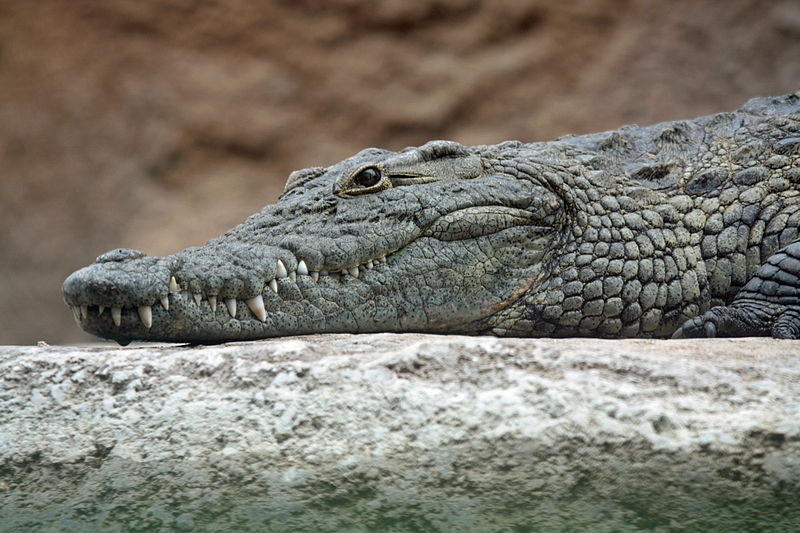
\includegraphics[width=0.5\textwidth]{crocodile.jpg}
\end{center}

\noindent Let us first see what happens when we use the arithmetic average. 
\begin{knitrout}
\definecolor{shadecolor}{rgb}{0.969, 0.969, 0.969}\color{fgcolor}\begin{kframe}
\begin{alltt}
\hlstd{R} \hlkwb{<-} \hlkwd{c}\hlstd{(}\hlnum{1}\hlstd{,} \hlnum{0.9}\hlstd{,} \hlnum{0.7}\hlstd{,} \hlnum{1.4}\hlstd{)}
\hlstd{Rari} \hlkwb{<-} \hlkwd{sum}\hlstd{(R)} \hlopt{/} \hlnum{4}
\hlstd{Rari}
\end{alltt}
\end{kframe}
\end{knitrout}

\noindent The Arithmetic average here is 1 so you would expect a population with this growth rate to remain constant. Check what is happenning:

\begin{knitrout}
\definecolor{shadecolor}{rgb}{0.969, 0.969, 0.969}\color{fgcolor}\begin{kframe}
\begin{alltt}
\hlstd{R2009}\hlkwb{<-}\hlnum{1}
\hlstd{N2009}\hlkwb{<-}\hlnum{100}
\hlstd{N2010}\hlkwb{<-}\hlstd{R2009}\hlopt{*}\hlstd{N2009}

\hlstd{R2010}\hlkwb{<-}\hlnum{0.9}
\hlstd{N2011}\hlkwb{<-}\hlstd{R2010}\hlopt{*}\hlstd{N2010}

\hlstd{R2011}\hlkwb{<-}\hlnum{0.7}
\hlstd{N2012}\hlkwb{<-}\hlstd{R2011}\hlopt{*}\hlstd{N2011}

\hlstd{R2012}\hlkwb{<-}\hlnum{1.4}
\hlstd{N2013}\hlkwb{<-}\hlstd{R2012}\hlopt{*}\hlstd{N2012}
\end{alltt}
\end{kframe}
\end{knitrout}
\noindent What is the population size in 2010, 2011, 2012 and 2013? Is your population constant on the long term as you would expect from a population with a growth rate of 1?

\noindent There is obviously something wrong with the arithmetic average. This is because with $\lambda$ we are multiplying the R with each other: $N_4=R_{2009} \cdot R_{2010} \cdot R_{2011} \cdot R_{2012} \cdot N_0$. Instead of the arithmetic average, we need a average such that
\begin{equation}
\bar R^4=R_{2009} \cdot R_{2010} \cdot R_{2011} \cdot R_{2012}
\end{equation}
\noindent So we just have to solve for $\bar R$. To do so, we take the fourth root on each side of our expression:
\begin{equation}
\bar{R}=\sqrt[4]{R_{2009} \cdot R_{2010} \cdot R_{2011} \cdot R_{2012}}.
\end{equation}
But $R_{2009}=\frac{N_{2010}}{N_{2009}}$, $R_{2010}=\frac{N_{2011}}{N_{2010}}$,  $R_{2011}=\frac{N_{2012}}{N_{2011}}$ and  $R_{2012}=\frac{N_{2013}}{N_{2012}}$. So we can re-write
\begin{equation}
\bar R=\sqrt[4]{\frac{N_{2010}}{N_{2009}} \cdot \frac{N_{2011}}{N_{2010}} \cdot \frac{N_{2012}}{N_{2011}} \cdot \frac{N_{2013}}{N_{2012}}}.
\end{equation}
Which can be simplified as
\begin{equation}
\bar R=\sqrt[4]{\frac{N_{2013}}{N_{2009}}}.
\end{equation}
\noindent We can generalise this to
\begin{equation}
\bar R=\sqrt[t]{\frac{N_{t}}{N_{0}}}.
\end{equation}
where $t$ is the last time step. Calculate the geometric mean, does this value make more sens than the arithmetric mean that we calculated before? 

%%%%%%%%%%%%%%%%%%%%%%%%%%%%%%%%%%%%%%%%%%%%%%%%%
%%%%%%% CONT. GROWTH
%%%%%%%%%%%%%%%%%%%%%%%%%%%%%%%%%%%%%%%%%%%%%%%%%
\section{Continous Population Growth}
So far, we looked at discrete population growth. This type of growth is suitable for describing the growth of populations which reproduce punctually, for example during one annual breeding period. To describe the growth of population such as bacteria, or humans, a continuous growth model is more appropriate. Instead of having a population punctually increasing with time, the population is constantly growing by an infinitesimally small change in population size. The change in population size over time is thus a constant ($r$) times the population size:
\begin{equation}
\frac{dN}{dt} = r\cdot N
\end{equation}
We have seen during the lecture that the solution to this differential equation is: 
\begin{equation}
N_t=N_0e^{rt} \label{eqdiff}
\end{equation}
\noindent where $r$ is the instantaneous rate of increase. If we know the population instantaneous rate of increase and the initial population size, we can project the population in the future.  
\vspace{1.5ex}
\begin{center}
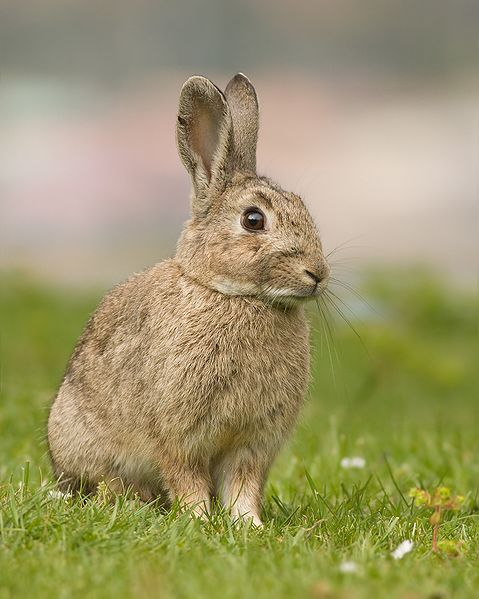
\includegraphics[width=0.5\textwidth]{Rabbit.jpg}
\end{center}

\noindent Let us look at a rabbit population in the UK. Rabbits have been introduced to the UK by the Romans and have since then proliferated. The rabbit population we consider breeds all year round and can be considered as continuously growing. The population currently is composed of 300 individuals with an instantaneous growth rate of 0.7. The wildlife management organisation want to know what the population will look like in 10 years.


To project this population with equation \ref{eqdiff}, we need the function \texttt{exp()}. This function returns the exponential of its input. Try \texttt{exp(1)} and \texttt{exp(2)}. These results correspond to $e^1$ and $e^2$ respectively. If you input a vector instead of a scalar into \texttt{exp()}, it will return a vector in which the first entry is the exponential of the first entry of the input vector. The second entry of the output vector will be the exponential of the second entry of the input vector:
\begin{knitrout}
\definecolor{shadecolor}{rgb}{0.969, 0.969, 0.969}\color{fgcolor}\begin{kframe}
\begin{alltt}
\hlkwd{exp}\hlstd{(}\hlkwd{c}\hlstd{(}\hlnum{1}\hlstd{,} \hlnum{2}\hlstd{))}
\end{alltt}
\end{kframe}
\end{knitrout}
The next step is to set the initial values of the UK rabbit population and write the equation for the expontial population growth in \texttt{R}.
\begin{knitrout}
\definecolor{shadecolor}{rgb}{0.969, 0.969, 0.969}\color{fgcolor}\begin{kframe}
\begin{alltt}
\hlstd{N0} \hlkwb{<-} \hlcom{#insert initial value here}
\hlstd{r} \hlkwb{<-}  \hlcom{#insert instantaneous rate of increase here }
\hlstd{t} \hlkwb{<-} \hlnum{0}\hlopt{:}\hlnum{10}
\hlstd{Nt} \hlkwb{<-} \hlstd{...}\hlopt{*}\hlkwd{exp}\hlstd{(...)}
\end{alltt}
\end{kframe}
\end{knitrout}
And then we plot the results. Because we are now considering a continuous growth, we are assuming that the population is not punctually increasing but constantly increasing. Thus instead of just plotting points, we can now plot a continuous line. This is what the last part (\verb+type="l"+) of the code does.
\begin{knitrout}
\definecolor{shadecolor}{rgb}{0.969, 0.969, 0.969}\color{fgcolor}\begin{kframe}
\begin{alltt}
\hlkwd{plot}\hlstd{(t, Nt,} \hlkwc{xlab}\hlstd{=}\hlstr{"time"}\hlstd{,} \hlkwc{ylab}\hlstd{=}\hlstr{"N"}\hlstd{,} \hlkwc{type}\hlstd{=}\hlstr{"l"}\hlstd{)}
\end{alltt}
\end{kframe}
\end{knitrout}

Do you think this is a realistic outcome? What mechanisms would prevent the population to grow like this in reality?


During the brief introduction to mathematics last week, we mentioned that the natural logarithm is the inverse function of the exponential. Plot $\ln(N_t)$ over time. The command in \texttt{R} for $\ln$ is \texttt{log()}. Do not forget to change the label of the y-axis. What is the slope of that line?
\begin{Exercise}[title=doubling time, label=dt, difficulty=2]
Solve on paper at what time step the rabbit population has doubled in size. For this you need to derive the formula for doubling time in a population with exponential growth. Start from equation \ref{eqdiff}. Compare your result with the graph in \texttt{R} to check your answer.
\end{Exercise}
\begin{Answer}[ref=dt]
We want to derive an equation for $t_{double}$ that is the time at which the population is twice the size of the initial population.
\begin{equation}
N_{t_{double}}=2N_0
\end{equation}
Substituting this expression into equation \ref{eqdiff} we get:
\begin{equation*}
2N_0=N_0e^{rt_{double}}
\end{equation*}
Now we need to solve for $t$. We start by dividing by $N_0$ which is on both sides of the equation.
\begin{equation*}
2=e^{rt_{double}}
\end{equation*}
Then we take the natural logarithm on each side to get ride of the exponential. 
\begin{equation*}
\ln(2)=rt_{double}
\end{equation*}
From there, the equation can be rearranged.
\begin{equation*}
\frac{\ln(2)}{r}=t_{double}
\end{equation*}
You can use \texttt{R} as a calculator to find the value of $t_{double}$ from the value of $r$ given at the begining of the section.
\begin{knitrout}
\definecolor{shadecolor}{rgb}{0.969, 0.969, 0.969}\color{fgcolor}\begin{kframe}
\begin{alltt}
\hlstd{r}\hlkwb{<-} \hlnum{0.7}
\hlstd{tdouble}\hlkwb{<-}\hlkwd{log}\hlstd{(}\hlnum{2}\hlstd{)}\hlopt{/}\hlstd{r}
\hlstd{tdouble}
\end{alltt}
\end{kframe}
\end{knitrout}
Even before a full year has passed, the population has already double in size.
\end{Answer}

\subsection{The link between continuous and discrete population growth}
Both the continuous and the discrete population growth describe the population size in the future, but what is the link between them?
Let us state each equation again:

\textit{continuous}
\begin{equation}
N_t=N_0e^{rt}\label{ec}
\end{equation}


\textit{discrete}
\begin{equation}
N_t=N_0\lambda^t \label{ed}
\end{equation}


Both equations \ref{ec} and \ref{ed} give the population growth at time $t$ so we can write:


\begin{equation}
N_0\lambda^t =N_0e^{rt}
\end{equation}

Solving for $\lambda$ we get:
\begin{equation}
\lambda =e^{r}
\end{equation}

This means that if you have $\lambda$, the finite rate of increase, you can calculate the instantaneous growth rate ($r$).

\section{Data Fitting}
So far, we have worked on simulated data. In this section we will work on real biological data. We will extract key population growth parameters and plot the data assuming 1) density-independence, 2) unlimited resources, 3) no environmental stochasticity and 4) no demographic stochasticity. The data you collected in the lab on the rotifer is not well suited for the type of population model that we covered during this practical.


Instead, we will examine the variation of a beaver population from Alberta, Canada from 1919 to 1981. The data is from \texttt{NERC Centre for Population Biology, Imperial College (1999) The Global Population Dynamics Database. http://www.sw.ic.ac.uk/cpb/cpb/gpdd.html} and was published in \textit{Furbearer harvests in North America, 1600-1984} by Novak, M., Obbard, M., Jones, J., Newman, R., Booth, A., Satterthwaite, A. \& Linscombe, G. in 1987.
\vspace{1.5ex}
\begin{center}
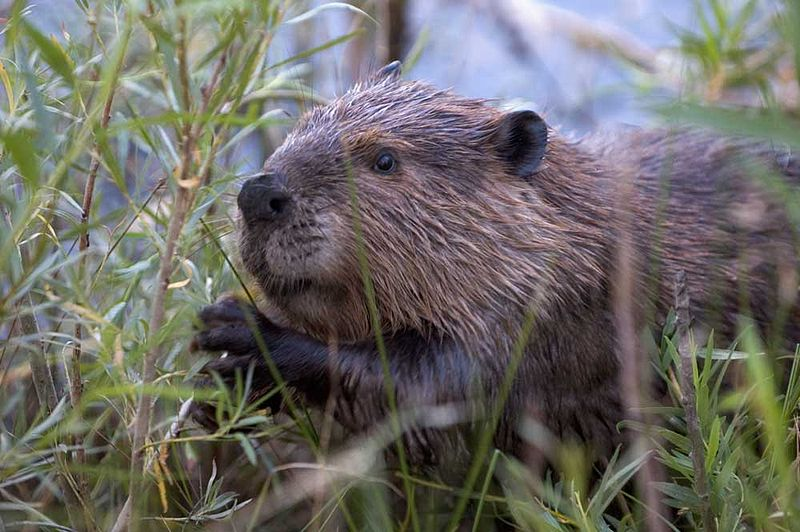
\includegraphics[height=0.35\textwidth]{Beaver.jpg}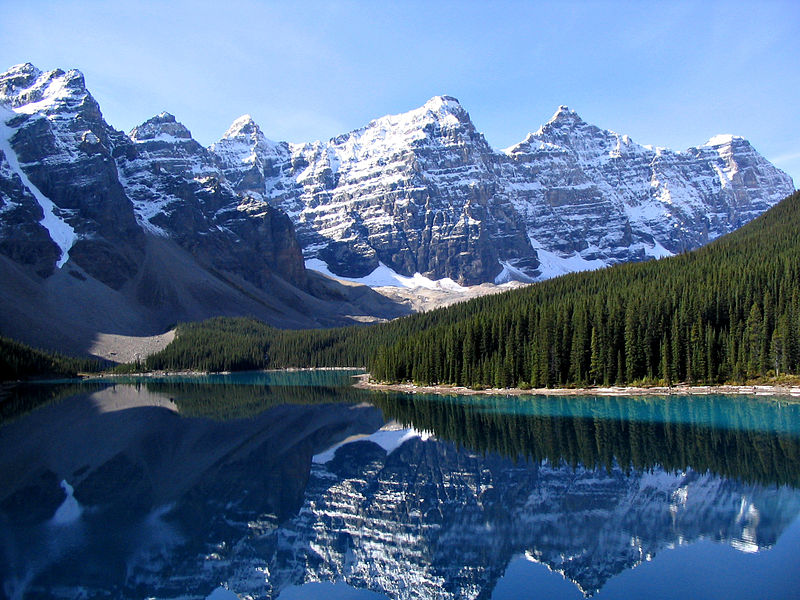
\includegraphics[height=0.35\textwidth]{Alberta.jpg}
\end{center}

First you need to take the \texttt{beaver\textunderscore pop.cvs} that we already put on OLAT and put it in a meaningful folder (for example the Pop\textunderscore Ecol folder on your desktop we created last time). As you now know, we 1) need to set the working directory and 2) open the file. Change the directory according to the location of your file.


\begin{knitrout}
\definecolor{shadecolor}{rgb}{0.969, 0.969, 0.969}\color{fgcolor}\begin{kframe}
\begin{alltt}
\hlkwd{setwd}\hlstd{(}\hlstr{"C:/Desktop/Pop_Ecol"}\hlstd{)}
\end{alltt}
\end{kframe}
\end{knitrout}

\begin{knitrout}
\definecolor{shadecolor}{rgb}{0.969, 0.969, 0.969}\color{fgcolor}\begin{kframe}
\begin{alltt}
\hlstd{Bea} \hlkwb{<-} \hlkwd{read.csv}\hlstd{(}\hlstr{"beaver_pop.csv"}\hlstd{,} \hlkwc{sep}\hlstd{=}\hlstr{";"}\hlstd{,} \hlkwc{header}\hlstd{=T)}
\hlkwd{head}\hlstd{(Bea)}
\hlkwd{str}\hlstd{(Bea)}
\end{alltt}
\end{kframe}
\end{knitrout}


The next step is to plot your data. Try to play around with the value of \texttt{scipen} to see how it effects the graph. What happens if it has a value of -1? If we set it once, it is remembered throughout the rest of the \texttt{R}-session.
\begin{knitrout}
\definecolor{shadecolor}{rgb}{0.969, 0.969, 0.969}\color{fgcolor}\begin{kframe}
\begin{alltt}
\hlkwd{options}\hlstd{(}\hlkwc{scipen}\hlstd{=}\hlnum{10}\hlstd{)}
\hlkwd{plot}\hlstd{(Bea}\hlopt{$}\hlstd{Year, Bea}\hlopt{$}\hlstd{Population,} \hlkwc{xlab}\hlstd{=}\hlstr{"year"}\hlstd{,} \hlkwc{ylab}\hlstd{=}\hlstr{"N"}\hlstd{)}
\end{alltt}
\end{kframe}
\end{knitrout}
It looks like this population may be decribed by an exponential function! 
\subsection{From the graph}
Let us try to find correct model parameters from the graph. To do so, we plot the natural logarithm of the population to see if there may be a linear relationship.
\begin{knitrout}
\definecolor{shadecolor}{rgb}{0.969, 0.969, 0.969}\color{fgcolor}\begin{kframe}
\begin{alltt}
\hlkwd{plot}\hlstd{(Bea}\hlopt{$}\hlstd{Year,} \hlkwd{log}\hlstd{(Bea}\hlopt{$}\hlstd{Population),} \hlkwc{xlab}\hlstd{=}\hlstr{"year"}\hlstd{,} \hlkwc{ylab}\hlstd{=}\hlstr{"ln(N)"}\hlstd{)}
\end{alltt}
\end{kframe}
\end{knitrout}
Remember that the straight line of the plot of the natural logarithm of the population is $r$, the instantaneous rate of increase. So we need to find the line that fits the points we just plotted. That means we want to fit a line for which the deviations of the actual data points to the line are minimized. This is a called a \textbf{linear regression}. The \texttt{lm} function fits a regression line through the points. If you type \verb+lm(N~t)+ it finds the line of the form $N=at+b$ that best describes the relation between $N$ and $t$. We however, want to fit a line through the natural logarithm of our points so we first transform them with the \texttt{log} function (we are thus looking for a line of the form $\ln(N)=at + b$). 
 
\begin{knitrout}
\definecolor{shadecolor}{rgb}{0.969, 0.969, 0.969}\color{fgcolor}\begin{kframe}
\begin{alltt}
\hlstd{reg1} \hlkwb{<-} \hlkwd{lm}\hlstd{(}\hlkwd{log}\hlstd{(Bea}\hlopt{$}\hlstd{Population)} \hlopt{~} \hlstd{Bea}\hlopt{$}\hlstd{Year)}
\hlstd{reg1} \hlcom{# Use this to take a look at reg1}
\end{alltt}
\end{kframe}
\end{knitrout}
And then we add the regression line on the graph.
\begin{knitrout}
\definecolor{shadecolor}{rgb}{0.969, 0.969, 0.969}\color{fgcolor}\begin{kframe}
\begin{alltt}
\hlkwd{abline}\hlstd{(reg1)}
\end{alltt}
\end{kframe}
\end{knitrout}
By running \texttt{reg1}, you see the outcome of the regression line. You get two coefficients; the intercept ($b$) and the slope ($a$, the value below \texttt{Bea\$Year}). These are the two values we want to find our exponential growth equation for this population.We have now an equation of the form 
\begin{equation}
\ln(N)=at+b
\end{equation}
Solving for N, we need to take the exponential on both sides of the equation which gives us $N=e^{at+b}$. This can also be writen as $N=e^b\cdot e^{at}$. Compare this to equation \ref{eqdiff}, and find $N_0$ and $r$.

Why is the initial population size for this equation not close to $5685$, the population size in 1919? 
%Because in the linear regression function, we stated that the initial year is year 0, and not 1919, the year at which the first data point for this population has been collected. So in fact our intercept gives us the size of this population in the year 0.

So we have found the values of the function:
\begin{equation}
N_t=N_{0}e^{rt}
\end{equation}

Let us now find the population size that would be predicted by the intercept and the slope we extracted from the linear regression. For this, use the commands \texttt{reg1\$coef[[1]]} and \texttt{reg1\$coef[[2]]}. 
\begin{knitrout}
\definecolor{shadecolor}{rgb}{0.969, 0.969, 0.969}\color{fgcolor}\begin{kframe}
\begin{alltt}
\hlstd{Bea}\hlopt{$}\hlstd{sim} \hlkwb{<-} \hlstd{...} \hlopt{*} \hlkwd{exp}\hlstd{(...} \hlopt{*} \hlstd{(Bea}\hlopt{$}\hlstd{Year))}
\end{alltt}
\end{kframe}
\end{knitrout}


And plot it on the same graph as the original population. 
\begin{knitrout}
\definecolor{shadecolor}{rgb}{0.969, 0.969, 0.969}\color{fgcolor}\begin{kframe}
\begin{alltt}
\hlkwd{plot}\hlstd{(Bea}\hlopt{$}\hlstd{Year, Bea}\hlopt{$}\hlstd{Population,} \hlkwc{xlab}\hlstd{=}\hlstr{"year"}\hlstd{,} \hlkwc{ylab}\hlstd{=}\hlstr{"N"}\hlstd{)}
\hlkwd{lines}\hlstd{(Bea}\hlopt{$}\hlstd{Year,  Bea}\hlopt{$}\hlstd{sim)}
\end{alltt}
\end{kframe}
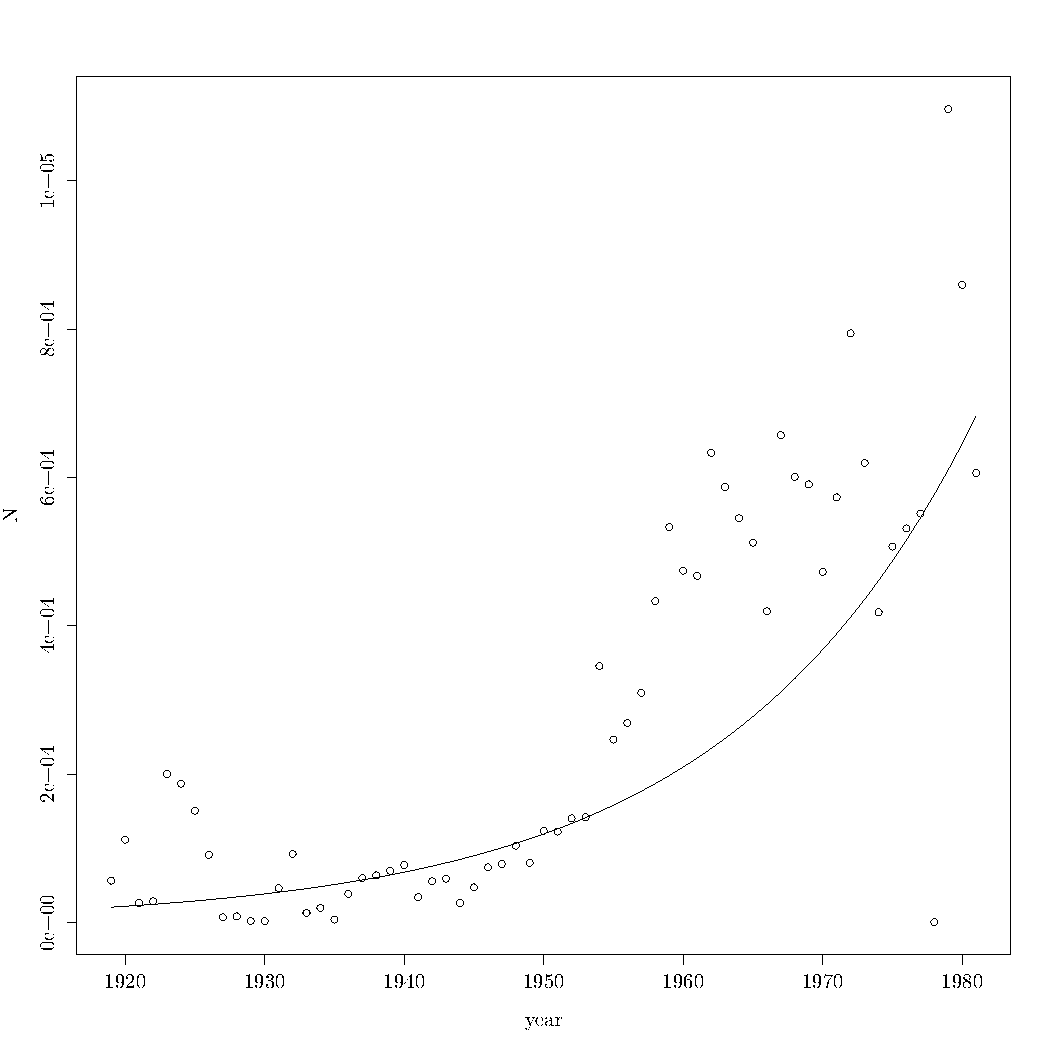
\includegraphics[width=\maxwidth]{figure/t25-1} 

\end{knitrout}
The fit is actually not bad at all!

\begin{Exercise}[title=fitting data from graph, label=fd, difficulty=2]
As an exercise, write down the exponential growth equation of this beaver population with the parameter values. Knowing the relationship between the finite rate of increase $\lambda$ and the instantenous growth rate $r$, find $\lambda$ and write the discrete population growth equation down. 

Show your equations to one of the instructors.
\end{Exercise}
\begin{Answer}[ref=fd]
$N_t=e^{\ensuremath{-100.248}}\cdot e^{0.056t}$

\begin{knitrout}
\definecolor{shadecolor}{rgb}{0.969, 0.969, 0.969}\color{fgcolor}\begin{kframe}
\begin{alltt}
\hlstd{lambda1}\hlkwb{<-}\hlkwd{exp}\hlstd{(reg1}\hlopt{$}\hlstd{coef[[}\hlnum{2}\hlstd{]])}
\hlstd{lambda1}
\end{alltt}
\begin{verbatim}
## [1] 1.057835
\end{verbatim}
\end{kframe}
\end{knitrout}
$\lambda=1.058$

$N_t=e^{\ensuremath{-100.248}}\cdot 1.058^t$
\end{Answer}
\subsection{More about the average growth rate}

An alternative to find the function describing the growth of this population is to go from the average growth rate which we will call $R$. In the section \textit{Average growth rate}, we showed that the average growth rate is given by $R=\sqrt[t]{\frac{N_t}{N_0}}$. The code \texttt{length} gives the number of elements of the object it is applied to. We take the length of our population variable $-1$ because among $n$ points, there are always $n-1$ transitions. Run separately the different parts of the code below to find out what they do.
\begin{knitrout}
\definecolor{shadecolor}{rgb}{0.969, 0.969, 0.969}\color{fgcolor}\begin{kframe}
\begin{alltt}
\hlstd{N0} \hlkwb{<-} \hlstd{Bea}\hlopt{$}\hlstd{Population[}\hlnum{1}\hlstd{]}
\hlstd{Nt} \hlkwb{<-} \hlstd{Bea}\hlopt{$}\hlstd{Population[}\hlkwd{length}\hlstd{(Bea}\hlopt{$}\hlstd{Population)]}

\hlstd{lambda} \hlkwb{<-} \hlstd{(Nt} \hlopt{/} \hlstd{N0)} \hlopt{^} \hlstd{(}\hlnum{1} \hlopt{/} \hlstd{(}\hlkwd{length}\hlstd{(Bea}\hlopt{$}\hlstd{Population)} \hlopt{-} \hlnum{1}\hlstd{))}
\hlstd{lambda}
\end{alltt}
\end{kframe}
\end{knitrout}

\begin{Exercise}[title=Comparing the $\lambda$s, label=fdd, difficulty=2]
Compare this value of lambda with the value of lambda you found in the former exercise. Knowing the relationship between the finite rate of increase $\lambda$ and the instantenous growth rate $r$, find $r$ and write the discrete and continuous population growth equations with the appropriate parameters

Show your equations to one of the instructors.
\end{Exercise}
\begin{Answer}[ref=fdd]
$N_t=5685\cdot 1.039^t$


$\lambda=1.039$
\begin{knitrout}
\definecolor{shadecolor}{rgb}{0.969, 0.969, 0.969}\color{fgcolor}\begin{kframe}
\begin{alltt}
\hlstd{r1}\hlkwb{<-}\hlkwd{log}\hlstd{(lambda)}
\hlstd{r1}
\end{alltt}
\begin{verbatim}
## [1] 0.03817303
\end{verbatim}
\end{kframe}
\end{knitrout}

$N_t=5685\cdot e^{0.038t}$

\end{Answer}
\vspace{1.5ex}
Let us compare the two curves we got with the different value of $\lambda$. For this we again use the same plotting code and an extra line.

\begin{knitrout}
\definecolor{shadecolor}{rgb}{0.969, 0.969, 0.969}\color{fgcolor}\begin{kframe}
\begin{alltt}
\hlkwd{plot}\hlstd{(Bea}\hlopt{$}\hlstd{Year, Bea}\hlopt{$}\hlstd{Population,} \hlkwc{xlab}\hlstd{=}\hlstr{"year"}\hlstd{,} \hlkwc{ylab}\hlstd{=}\hlstr{"N"}\hlstd{)}
\hlkwd{options}\hlstd{(}\hlkwc{scipen}\hlstd{=}\hlnum{10}\hlstd{)}
\hlkwd{lines}\hlstd{(Bea}\hlopt{$}\hlstd{Year,  Bea}\hlopt{$}\hlstd{sim)} \hlcom{#line from the linear regression}
\hlkwd{lines}\hlstd{(Bea}\hlopt{$}\hlstd{Year,Bea}\hlopt{$}\hlstd{Population[}\hlnum{1}\hlstd{]}\hlopt{*}
        \hlstd{lambda}\hlopt{^}\hlstd{(}\hlnum{0}\hlopt{:}\hlstd{(}\hlkwd{length}\hlstd{(Bea}\hlopt{$}\hlstd{Population)}\hlopt{-}\hlnum{1}\hlstd{))}
      \hlstd{,}\hlkwc{col}\hlstd{=}\hlstr{'red'}\hlstd{)} \hlcom{#line from the average growth rate}
\end{alltt}
\end{kframe}
\end{knitrout}

You can see that the two curves are not identical. This is because of the methods we used to estimate $\lambda$. The curve from the linear regression is a fit. The average distance between the data points and the line is minimized. You can see that the curve neither starts nor ends at one of the data points. However the curve obtained from the average growth rate is a mean and does starts at the first data point and ends on the last data point of the serie. To convince you of this, let us repeat both analyses on a subset of the dataset where the last three points are excluded. 
\begin{knitrout}
\definecolor{shadecolor}{rgb}{0.969, 0.969, 0.969}\color{fgcolor}\begin{kframe}
\begin{alltt}
\hlstd{Beasub}\hlkwb{<-}\hlstd{Bea[}\hlnum{1}\hlopt{:}\hlnum{60}\hlstd{,]}

\hlcom{#From the fit}
\hlstd{reg2} \hlkwb{<-} \hlkwd{lm}\hlstd{(}\hlkwd{log}\hlstd{(Beasub}\hlopt{$}\hlstd{Population)}\hlopt{~}\hlstd{Beasub}\hlopt{$}\hlstd{Year)}
\hlstd{Beasub}\hlopt{$}\hlstd{sim}\hlkwb{<-}\hlkwd{exp}\hlstd{( reg2}\hlopt{$}\hlstd{coef[[}\hlnum{1}\hlstd{]])}\hlopt{*}\hlkwd{exp}\hlstd{( reg2}\hlopt{$}\hlstd{coef[[}\hlnum{2}\hlstd{]]}\hlopt{*}\hlstd{(Beasub}\hlopt{$}\hlstd{Year))}

\hlcom{#From the average growth rate}
\hlstd{N02}\hlkwb{<-}\hlstd{Beasub}\hlopt{$}\hlstd{Population[}\hlnum{1}\hlstd{]}
\hlstd{Nt2}\hlkwb{<-}\hlstd{Beasub}\hlopt{$}\hlstd{Population[}\hlkwd{length}\hlstd{(Beasub}\hlopt{$}\hlstd{Population)]}

\hlstd{lambda2}\hlkwb{<-}\hlstd{(Nt2}\hlopt{/}\hlstd{N02)}\hlopt{^}\hlstd{(}\hlnum{1}\hlopt{/}\hlstd{(}\hlkwd{length}\hlstd{(Beasub}\hlopt{$}\hlstd{Population)}\hlopt{-}\hlnum{1}\hlstd{))}
\hlstd{lambda2}
\end{alltt}
\begin{verbatim}
## [1] 0.9279561
\end{verbatim}
\begin{alltt}
\hlcom{#The plots }
\hlkwd{plot}\hlstd{(Bea}\hlopt{$}\hlstd{Year, Bea}\hlopt{$}\hlstd{Population,} \hlkwc{xlab}\hlstd{=}\hlstr{"year"}\hlstd{,} \hlkwc{ylab}\hlstd{=}\hlstr{"$N$"}\hlstd{)}
\hlkwd{options}\hlstd{(}\hlkwc{scipen}\hlstd{=}\hlnum{10}\hlstd{)}
\hlkwd{lines}\hlstd{(Bea}\hlopt{$}\hlstd{Year,  Bea}\hlopt{$}\hlstd{sim,} \hlkwc{col}\hlstd{=}\hlstr{'black'}\hlstd{)}
\hlkwd{lines}\hlstd{(Bea}\hlopt{$}\hlstd{Year,Bea}\hlopt{$}\hlstd{Population[}\hlnum{1}\hlstd{]}\hlopt{*}\hlstd{lambda}\hlopt{^}\hlstd{(}
  \hlnum{0}\hlopt{:}\hlstd{(}\hlkwd{length}\hlstd{(Bea}\hlopt{$}\hlstd{Population)}\hlopt{-}\hlnum{1}\hlstd{)),}\hlkwc{col}\hlstd{=}\hlstr{'red'}\hlstd{)}

\hlkwd{lines}\hlstd{(Beasub}\hlopt{$}\hlstd{Year,  Beasub}\hlopt{$}\hlstd{sim,} \hlkwc{col}\hlstd{=}\hlstr{'black'}\hlstd{,} \hlkwc{lty}\hlstd{=}\hlnum{2}\hlstd{)}
\hlkwd{lines}\hlstd{(Beasub}\hlopt{$}\hlstd{Year,Beasub}\hlopt{$}\hlstd{Population[}\hlnum{1}\hlstd{]}\hlopt{*}\hlstd{lambda2}\hlopt{^}\hlstd{(}
  \hlnum{0}\hlopt{:}\hlstd{(}\hlkwd{length}\hlstd{(Beasub}\hlopt{$}\hlstd{Population)}\hlopt{-}\hlnum{1}\hlstd{)),}\hlkwc{col}\hlstd{=}\hlstr{'red'}\hlstd{,} \hlkwc{lty}\hlstd{=}\hlnum{2}\hlstd{)}
\hlkwd{legend}\hlstd{(}\hlstr{"topleft"}\hlstd{,}
       \hlkwd{c}\hlstd{(}\hlstr{"fit full "}\hlstd{,}\hlstr{"fit subset"}\hlstd{,} \hlstr{"avg full"}\hlstd{,} \hlstr{"avg subset"}\hlstd{),}
       \hlkwc{bty} \hlstd{=} \hlstr{"n"}\hlstd{,}
\hlkwc{lty}\hlstd{=}\hlkwd{c}\hlstd{(}\hlnum{1}\hlstd{,}\hlnum{2}\hlstd{,}\hlnum{1}\hlstd{,}\hlnum{2}\hlstd{),}
\hlkwc{col}\hlstd{=}\hlkwd{c}\hlstd{(}\hlstr{"black"}\hlstd{,} \hlstr{"black"}\hlstd{,} \hlstr{"red"}\hlstd{,} \hlstr{"red"}\hlstd{))}
\end{alltt}
\end{kframe}

{\centering 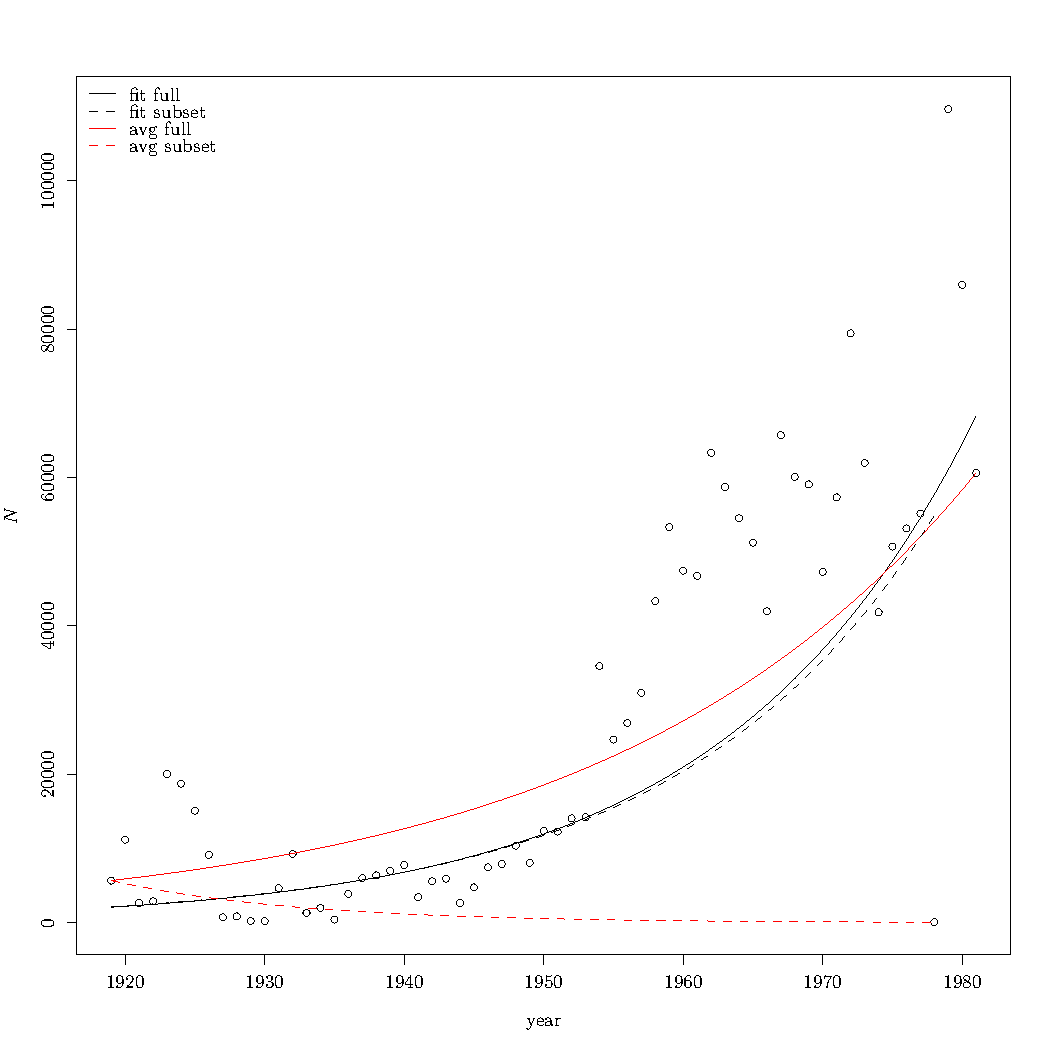
\includegraphics[width=0.65\textwidth]{figure/t30-1} 

}



\end{knitrout}
When the last three points have been removed, the last point is a particularily low value. You can see in this case that the $\lambda$ from the average growth rate causes the projected population to be far from the actual population trajectory because the curve goes through both the first and the last point. In contrast, the two curves issued from the projections from the $\lambda$ from the linear regressions are not very different from each other. The last and first data points have much less influence on their behaviour. 



\section{Logistic Growth}
\subsection{Continuous Logistic Model}
So far we have assumed that the rabbits have a constant growth rate (where we found that $r=0.7$), regardless of the population size. In reality however, this growth rate is the maximum possible growth rate. In larger populations the actual growth rate is smaller than this maximal value (due to competition for food). Below we show how the growth rate depends on the population size: 

\begin{knitrout}
\definecolor{shadecolor}{rgb}{0.969, 0.969, 0.969}\color{fgcolor}

{\centering 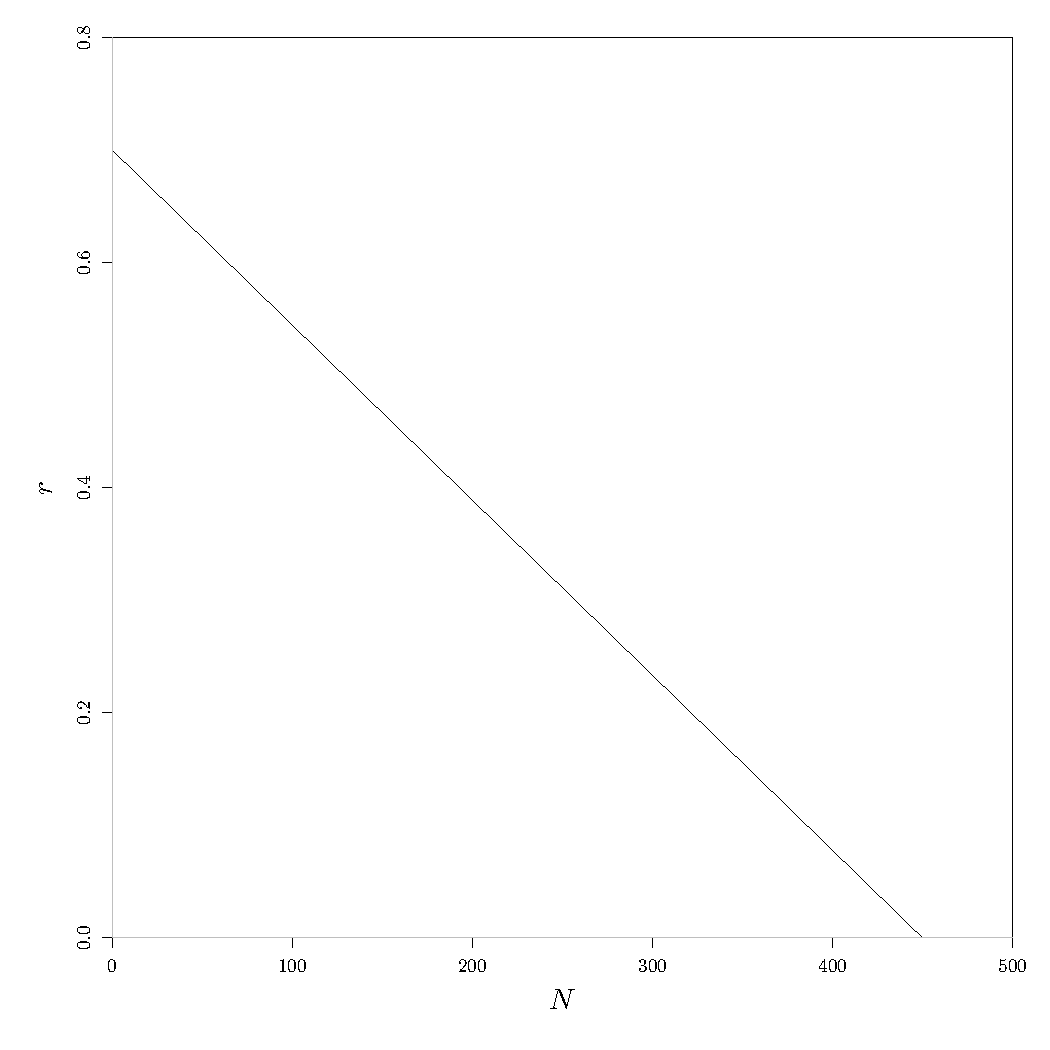
\includegraphics[width=0.7\textwidth]{figure/k1-1} 

}



\end{knitrout}
From this graph, find the carrying capacity ($K$) of this population and set it in \texttt{R}:
\begin{knitrout}
\definecolor{shadecolor}{rgb}{0.969, 0.969, 0.969}\color{fgcolor}\begin{kframe}
\begin{alltt}
K <-
\end{alltt}
\end{kframe}
\end{knitrout}
What is the population growth rate when the population size equals the carrying capacity?
\begin{equation*}
r(K) = \dots
\end{equation*}
Think about what this means for the population size when it reaches the carrying capacity.

In the lecture we saw that when the growth rate decreases linearly with the population size, the population can be described by logistic growth:
\begin{equation}
N = \frac{K}{1+\frac{K-N_0}{N_0}e^{-r_{max}t}}.
\label{keq02}
\end{equation}
Now we will use \texttt{R} to see how changes in $K$, $N_0$ and $r_{max}$ influence the population size over time. First we need to create a vector in \texttt{R} that contains the time values at which we want to evaluate $N(t)$. For this exercise, let us use the time vector:
\begin{equation*}
\texttt{time} = \texttt{c(} 0, 0.1, 0.2, 0.3, \dots 10\texttt{)}
\end{equation*}
Use the function \texttt{seq()} to make this vector in \texttt{R}. Type \texttt{?seq} in the console if you do not know how the function \texttt{seq()} works.
\begin{knitrout}
\definecolor{shadecolor}{rgb}{0.969, 0.969, 0.969}\color{fgcolor}\begin{kframe}
\begin{alltt}
\hlstd{time}\hlkwb{<-}\hlkwd{seq}\hlstd{(    ,   ,   )}
\end{alltt}
\end{kframe}
\end{knitrout}

\noindent Check your vector by outputting the first and the last few entries of \texttt{time}:
\begin{knitrout}
\definecolor{shadecolor}{rgb}{0.969, 0.969, 0.969}\color{fgcolor}\begin{kframe}
\begin{alltt}
\hlkwd{head}\hlstd{(time)}
\end{alltt}
\begin{verbatim}
## [1] 0.0 0.1 0.2 0.3 0.4 0.5
\end{verbatim}
\begin{alltt}
\hlkwd{tail}\hlstd{(time)}
\end{alltt}
\begin{verbatim}
## [1]  9.5  9.6  9.7  9.8  9.9 10.0
\end{verbatim}
\end{kframe}
\end{knitrout}
Now we will calculate the values of $N$ at these times. To do so we need the function \texttt{exp()}. Like before, we assume that the population size starts with $300$ individuals. In order to find the population size $N$ at all the time points in \texttt{time}, complete the following code:
\begin{knitrout}
\definecolor{shadecolor}{rgb}{0.969, 0.969, 0.969}\color{fgcolor}\begin{kframe}
\begin{alltt}
\hlstd{K} \hlkwb{<-}     \hlcom{# Input your value of K here}
\hlstd{rmax} \hlkwb{<-}  \hlcom{# Input the value of rmax here}
\hlstd{N0} \hlkwb{<-} \hlnum{300}
\hlstd{N} \hlkwb{<-} \hlstd{K} \hlopt{/} \hlstd{(...} \hlopt{*} \hlkwd{exp}\hlstd{(...} \hlopt{*} \hlstd{time))}
\end{alltt}
\end{kframe}
\end{knitrout}

Now we plot the behaviour of $N$ against time:
\begin{knitrout}
\definecolor{shadecolor}{rgb}{0.969, 0.969, 0.969}\color{fgcolor}\begin{kframe}
\begin{alltt}
\hlkwd{plot}\hlstd{(time, N,} \hlkwc{ylab}\hlstd{=}\hlstr{"N"}\hlstd{,} \hlkwc{xlab}\hlstd{=}\hlstr{"t"}\hlstd{,} \hlkwc{type}\hlstd{=}\hlstr{"l"}\hlstd{,} \hlkwc{ylim}\hlstd{=}\hlkwd{c}\hlstd{(}\hlnum{200}\hlstd{,}\hlnum{500}\hlstd{))}
\end{alltt}
\end{kframe}
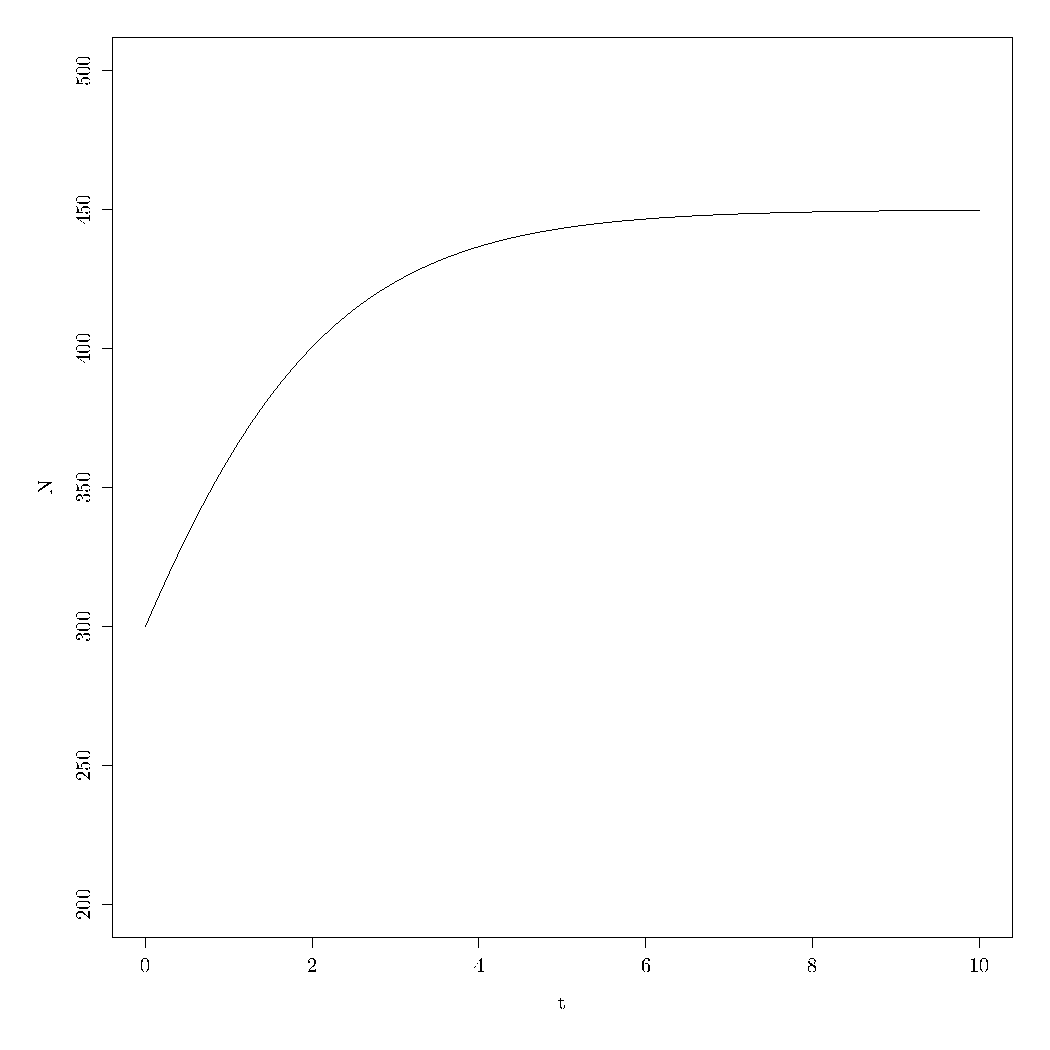
\includegraphics[width=\maxwidth]{figure/k9-1} 

\end{knitrout}
Now change one of the parameters ($K,r_{max},N0$) and calculate the new values for $N$. Next, you can add a line with these new values to your current plot by using the function \texttt{lines()}. Below the code is illustrated for a change in the initial population size ($N_0$):
\begin{knitrout}
\definecolor{shadecolor}{rgb}{0.969, 0.969, 0.969}\color{fgcolor}\begin{kframe}
\begin{alltt}
\hlstd{N0} \hlkwb{<-} \hlnum{350}
\hlstd{N} \hlkwb{<-} \hlstd{K} \hlopt{/} \hlstd{(...} \hlopt{*} \hlkwd{exp}\hlstd{(...} \hlopt{*} \hlstd{time))}
\hlkwd{lines}\hlstd{(time,N,}\hlkwc{col}\hlstd{=}\hlstr{"red"}\hlstd{)}
\end{alltt}
\end{kframe}
\end{knitrout}
Now change $r_{max}$ and $K$ and see how they influence the behaviour of the population. \textbf{If you want to compare the changed situation to the original one, do not forget to set $N_0$ back at its original value. You may consider writing a function that returns N.} What do the different parameters ($N_0,r_{max}, K$) determine? What happens if $K<N_0$? And what do you see if $N_0 < \frac{K}{2}$? \textit{Make sure to adjust the parameter} \texttt{ylim} \textit{in your plot if necessary.}

We conclude this exercise on continuous logistic growth with a \textit{pen \& paper} exercise:
\begin{Exercise}[title=Logistic Growth,label=kloge1,difficulty=2]
\noindent In the lecture Arpat talked about density dependent population growth. He showed that if the growth rate of the population depends linearly on the number of individuals, the following equation holds:
\begin{equation}
\frac{dN}{dt} = r_{max} N \left( 1-\frac{N}{K}\right).
\label{keq1}
\end{equation}
He also showed that the solution to this equation is:
\begin{equation}
N = \frac{K}{1+\frac{K-N_0}{N_0}e^{-r_{max}t}}.
\label{keq2}
\end{equation}
From this equation calculate separately $\frac{dN}{dt}$ and  $r_{max} N \left( 1-\frac{N}{K}\right) $ and show that the two are equal. Hereby you show that equation \ref{keq2} is indeed the solution to equation \ref{keq1}.

\end{Exercise}

\begin{Answer}[ref=kloge1]
Let us first consider $\frac{dN}{dt}$. First we write:
\begin{align*}
N(u) &= \frac{K}{u} = Ku^{-1} & u(t) = 1+\frac{K-N_0}{N_0}e^{-r_{max}t}
\end{align*}
From this we can find:
\begin{align*}
N^\prime(u) &= - K u^{-2} & u^\prime(t) = -\frac{K-N_0}{N_0}r_{max}e^{-r_{max}t} 
\end{align*}
We know the chain rule: $N^\prime(t) = N^\prime(u) u^\prime(t)$, so:
\begin{equation*}
\frac{dN}{dt} = K u^{-2} \frac{K-N_0}{N_0}r_{max}e^{-r_{max}t} 
\end{equation*}
Substituting $u$:
\begin{equation*}
\frac{dN}{dt} = \frac{\frac{K-N_0}{N_0} K r_{max}e^{-r_{max}t}}{(1+\frac{K-N_0}{N_0}e^{-r_{max}t})^{2}} 
\end{equation*}
Now we consider the righthand side of the equation: $r_{max} N \left( 1-\frac{N}{K}\right) $. We fill in the solution for $N$:
\begin{align*}
r_{max} N \left( 1-\frac{N}{K}\right) &= r_{max} \frac{K}{1+\frac{K-N_0}{N_0}e^{-r_{max}t}} \left( 1-\frac{1}{1+\frac{K-N_0}{N_0}e^{-r_{max}t}}\right) \\ &= r_{max} \frac{K}{1+\frac{K-N_0}{N_0}e^{-r_{max}t}} \left( \frac{1+\frac{K-N_0}{N_0}e^{-r_{max}t}}{1+\frac{K-N_0}{N_0}e^{-r_{max}t}}-\frac{1}{1+\frac{K-N_0}{N_0}e^{-r_{max}t}}\right)\\ &= r_{max} \frac{K}{1+\frac{K-N_0}{N_0}e^{-r_{max}t}} \left( \frac{\frac{K-N_0}{N_0}e^{-r_{max}t}}{1+\frac{K-N_0}{N_0}e^{-r_{max}t}}\right)\\ &= \frac{K r_{max}\frac{K-N_0}{N_0}e^{-r_{max}t}}{(1+\frac{K-N_0}{N_0}e^{-r_{max}t})^2}
\end{align*}
Comparing this outcome with the expression for $\frac{dN}{dt}$, we see that the two are equivalent and thus that equation \ref{keq2} satisfies equation \ref{keq1}. Arpat was thus correct when he told us this!
\vspace{1.5ex}
\end{Answer}
\subsection{Discrete Logistic Growth Model}
Now we will consider the discrete logistic growth model (Ricker's version, see lecture):
\begin{equation}
N_{t+1} = N_t e^{\left(r_{d}\left[1-\frac{N_t}{K}\right]\right)}.
\end{equation}

\vspace{1.5ex}

\begin{center}
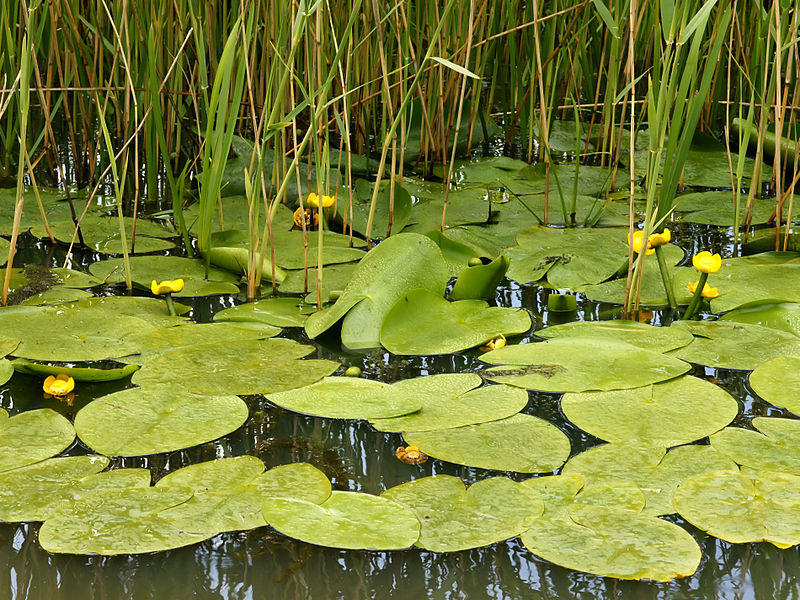
\includegraphics[width=0.65\textwidth]{Pond_lily.jpg}
\end{center}
\vspace{1.5ex}

Let us consider again the pond-lily example. The botanical garden decided to create a second, larger pond where they put $300$ individuals ($N_1 = 300$). The growth rate of this new population is $0.2$ and has a carrying capacity at $K=400$. Let us set these variable in \texttt{R}:
\begin{knitrout}
\definecolor{shadecolor}{rgb}{0.969, 0.969, 0.969}\color{fgcolor}\begin{kframe}
\begin{alltt}
\hlstd{N1} \hlkwb{<-} \hlnum{300}
\hlstd{rd} \hlkwb{<-} \hlnum{0.2}
\hlstd{K} \hlkwb{<-} \hlnum{400}
\end{alltt}
\end{kframe}
\end{knitrout}
Now from these numbers, calculate the population size at $t=2$ (that is, we want to calculate $N_2$). Now also calculate $N_3$ and $N_4$. The answers are shown below, so you can check them:\\
$N_2 =  315.4 $\\$N_3 =  329 $\\$N_4 =  340.9 $

If we want to know what the population size is at $t=100$, it is a bit inconvenient to manually calculate $N_2$ up to $N_{100}$ manually. So let's try to automatize that calculation. First we create a vector \texttt{N} with only zeros, in the end we will put the values of $N_1$ up to and including $N_{100}$ in this vector. Now create a vector with $100$ entries where every entry is zero. For this use the function \texttt{rep()}, if you do not know how this function works, use \texttt{?rep} to obtain more information on the function

Verify that the vector indeed has the desired length and that it contains zeros: 
\begin{knitrout}
\definecolor{shadecolor}{rgb}{0.969, 0.969, 0.969}\color{fgcolor}\begin{kframe}
\begin{alltt}
\hlkwd{length}\hlstd{(N)}
\end{alltt}
\begin{verbatim}
## [1] 100
\end{verbatim}
\begin{alltt}
\hlkwd{head}\hlstd{(N)}
\end{alltt}
\begin{verbatim}
## [1] 0 0 0 0 0 0
\end{verbatim}
\end{kframe}
\end{knitrout}
We already know the population size at the first position, so we can fill in the value of the first value:
\begin{knitrout}
\definecolor{shadecolor}{rgb}{0.969, 0.969, 0.969}\color{fgcolor}\begin{kframe}
\begin{alltt}
\hlstd{N[}\hlnum{1}\hlstd{]} \hlkwb{<-} \hlnum{300}

\hlkwd{head}\hlstd{(N)}
\end{alltt}
\begin{verbatim}
## [1] 300   0   0   0   0   0
\end{verbatim}
\end{kframe}
\end{knitrout}
Now we need to calculate the other entries of \texttt{N}, to do so we use a \textit{for-loop}. Below is an incomplete version of the code, please complete it and run the code to fill \texttt{N} with the correct values:
\begin{knitrout}
\definecolor{shadecolor}{rgb}{0.969, 0.969, 0.969}\color{fgcolor}\begin{kframe}
\begin{alltt}
\hlkwa{for}\hlstd{(i} \hlkwa{in} \hlnum{2}\hlopt{:}\hlstd{..)\{}
  \hlstd{N[i]} \hlkwb{<-} \hlstd{N[i}\hlopt{-}\hlstd{..]} \hlopt{*} \hlkwd{exp}\hlstd{(....)}
\hlstd{\}}
\end{alltt}
\end{kframe}
\end{knitrout}

Check the final vector to see that the values that were calculated in this way for the first few entries equal the values that you found earlier by manual calculation. Now we can easily retrieve the population size at $t=100$. Now plot how the population develops over time.
\begin{knitrout}
\definecolor{shadecolor}{rgb}{0.969, 0.969, 0.969}\color{fgcolor}\begin{kframe}
\begin{alltt}
\hlstd{N[}\hlnum{100}\hlstd{]}
\end{alltt}
\begin{verbatim}
## [1] 400
\end{verbatim}
\end{kframe}

{\centering 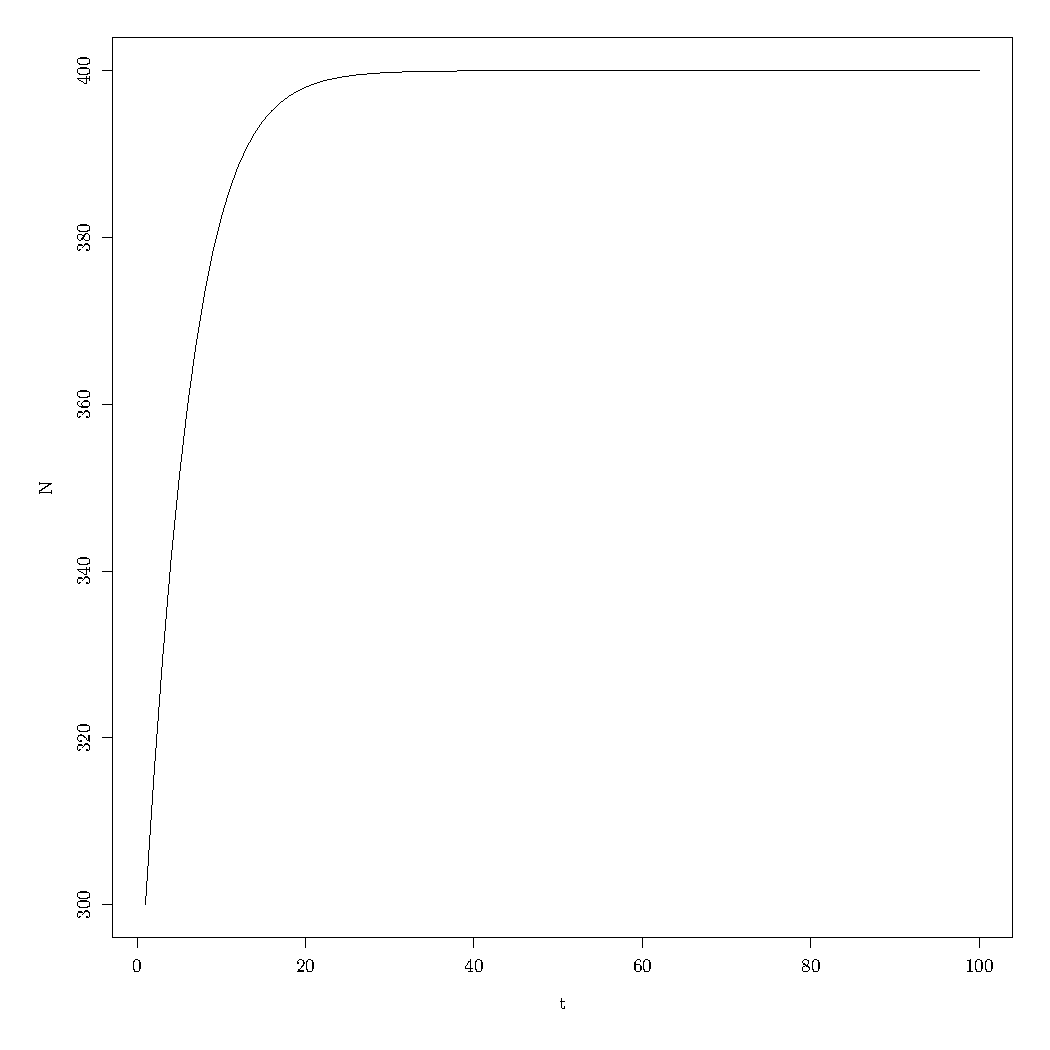
\includegraphics[width=0.65\textwidth]{figure/k18-1} 

}



\end{knitrout}
Run the model again with different values of $r_d$, can you explain why the model behaves strangely for large values of $r_d$ (e.g. $r_d=6$)?

\subsection{Environmental Stochasticity}
So far we have assumed that the growth rate $r_d$ and $K$ remain constant over time. In reality however, environmental influences will lead to these rates being different every year. We will incorporate this stochasticity in the model for the second pond-lily population and see how this influences the predictions of the model.

\subsubsection{Random numbers}
In order to incorporate this, we need random numbers. In \texttt{R} functions are available to generate pseudo random numbers from different distributions. One such function is \texttt{runif(N)}, this function generates $N$ random numbers between $0$ and $1$, where every number between $0$ and $1$ is equally likely to be drawn (the distribution is uniform).
\begin{knitrout}
\definecolor{shadecolor}{rgb}{0.969, 0.969, 0.969}\color{fgcolor}\begin{kframe}
\begin{alltt}
\hlkwd{runif}\hlstd{(}\hlnum{7}\hlstd{)}
\end{alltt}
\begin{verbatim}
## [1] 0.43684728 0.20360383 0.60170333 0.46655214 0.05392449
## [6] 0.40150360 0.21442341
\end{verbatim}
\begin{alltt}
\hlkwd{hist}\hlstd{(}\hlkwd{runif}\hlstd{(}\hlnum{10000}\hlstd{),}\hlkwc{n}\hlstd{=}\hlnum{20}\hlstd{,}\hlkwc{main}\hlstd{=}\hlstr{""}\hlstd{,}
     \hlkwc{xlab}\hlstd{=}\hlstr{"value of $10.000$ random numbers"}\hlstd{,} \hlkwc{cex.lab}\hlstd{=}\hlnum{1.5}\hlstd{)}
\end{alltt}
\end{kframe}

{\centering 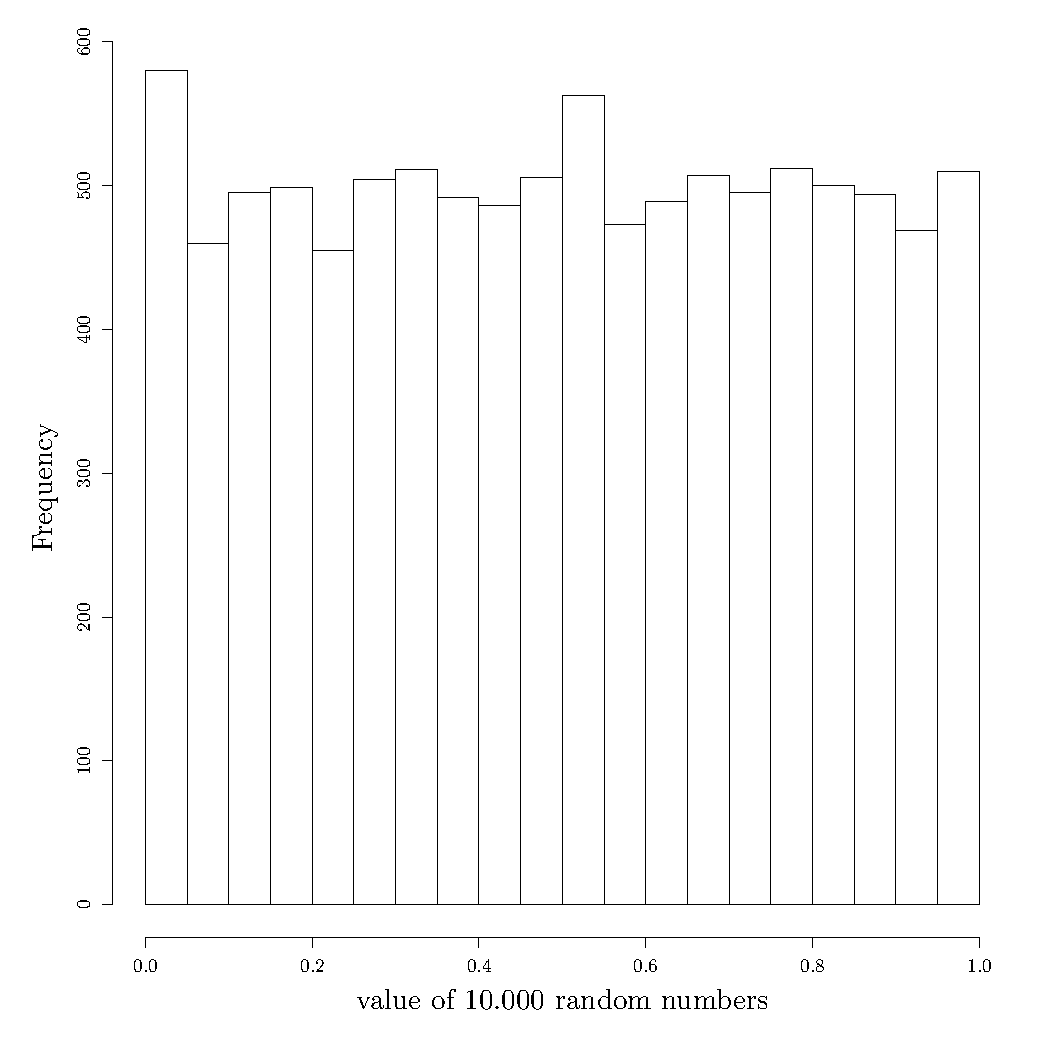
\includegraphics[width=0.5\textwidth]{figure/k19-1} 

}



\end{knitrout}
A computer works in a deterministic way, it is therefore not able to generate truly random numbers. Some algorithms have been developed however that generate series of numbers that very strongly resemble random numbers. They are not truly random: they depend on an initial number which is called the seed. If the seed is set to the same value, \texttt{R} will generate the same random numbers. The seed can be set by using the function \texttt{set.seed()}. When you use \texttt{R} for generating a random number, without explicitly setting the seed during an \texttt{R-}session, the seed is generated from the current time on your computer and the process ID. Compare the following lines of code:
\begin{knitrout}
\definecolor{shadecolor}{rgb}{0.969, 0.969, 0.969}\color{fgcolor}\begin{kframe}
\begin{alltt}
\hlkwd{set.seed}\hlstd{(}\hlnum{24}\hlstd{)}
\hlkwd{runif}\hlstd{(}\hlnum{7}\hlstd{)}
\end{alltt}
\begin{verbatim}
## [1] 0.2925740 0.2248911 0.7042230 0.5188971 0.6626196
## [6] 0.9204438 0.2797356
\end{verbatim}
\begin{alltt}
\hlkwd{runif}\hlstd{(}\hlnum{7}\hlstd{)}
\end{alltt}
\begin{verbatim}
## [1] 0.7638205 0.8016306 0.2547251 0.6048889 0.3707349
## [6] 0.6716903 0.6729823
\end{verbatim}
\begin{alltt}
\hlkwd{set.seed}\hlstd{(}\hlnum{24}\hlstd{)}
\hlkwd{runif}\hlstd{(}\hlnum{7}\hlstd{)}
\end{alltt}
\begin{verbatim}
## [1] 0.2925740 0.2248911 0.7042230 0.5188971 0.6626196
## [6] 0.9204438 0.2797356
\end{verbatim}
\end{kframe}
\end{knitrout}
More random numbers than this can be obtained from \texttt{www.random.org}. This website generates random numbers based on atmospheric noise. For most simulation purposes, however, pseudo random number generators are good enough.

A second function for generating random numbers is the function \texttt{rnorm()}, use this function to create a histogram for $10.000$ random numbers with a standard deviation and mean of your choice. If you are not familiar with this function, use \texttt{?rnorm} to obtain more information on this function.

\subsubsection{Environmental Stochasticity in the Logistic Growth Model}

We will now use such random numbers to simulate environmental stochasticity in the logistic growth model. Before we assumed that both $r$ and $K$ were the same every timestep. Instead of assuming this, we will now assume that every timestep these parameters are drawn from a normal distribution. Back to the pond-lily population, for $r_d$ the mean of this distribution is $\mu=0.2$ and the standard deviation $\sigma = 0.1$. For $K$ we take a normal distribution with mean $\mu=400$ and standard deviation $\sigma = 25$. Now adapt the code for the discrete logistic growth model to draw 1 new value for both $K$ and $r_d$ every time step and using these values to calculate the population numbers. We start with a population size of $300$. Plotting the final result may look like this (depending on your random numbers of course...):
\begin{knitrout}
\definecolor{shadecolor}{rgb}{0.969, 0.969, 0.969}\color{fgcolor}

{\centering 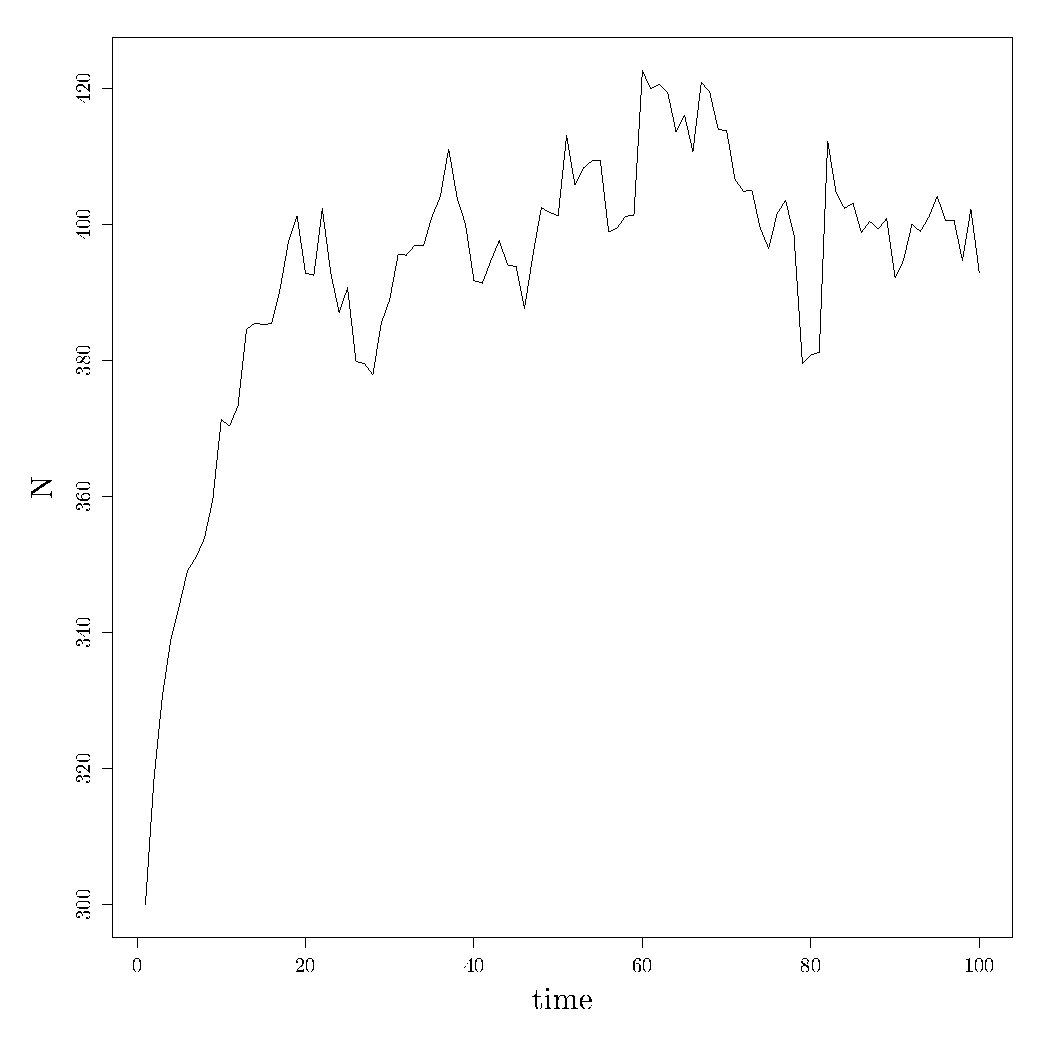
\includegraphics[width=0.65\textwidth]{figure/k21-1} 

}



\end{knitrout}
Now we will make a plot that shows multiple possible outcomes of the logistic growth:
\begin{knitrout}
\definecolor{shadecolor}{rgb}{0.969, 0.969, 0.969}\color{fgcolor}

{\centering 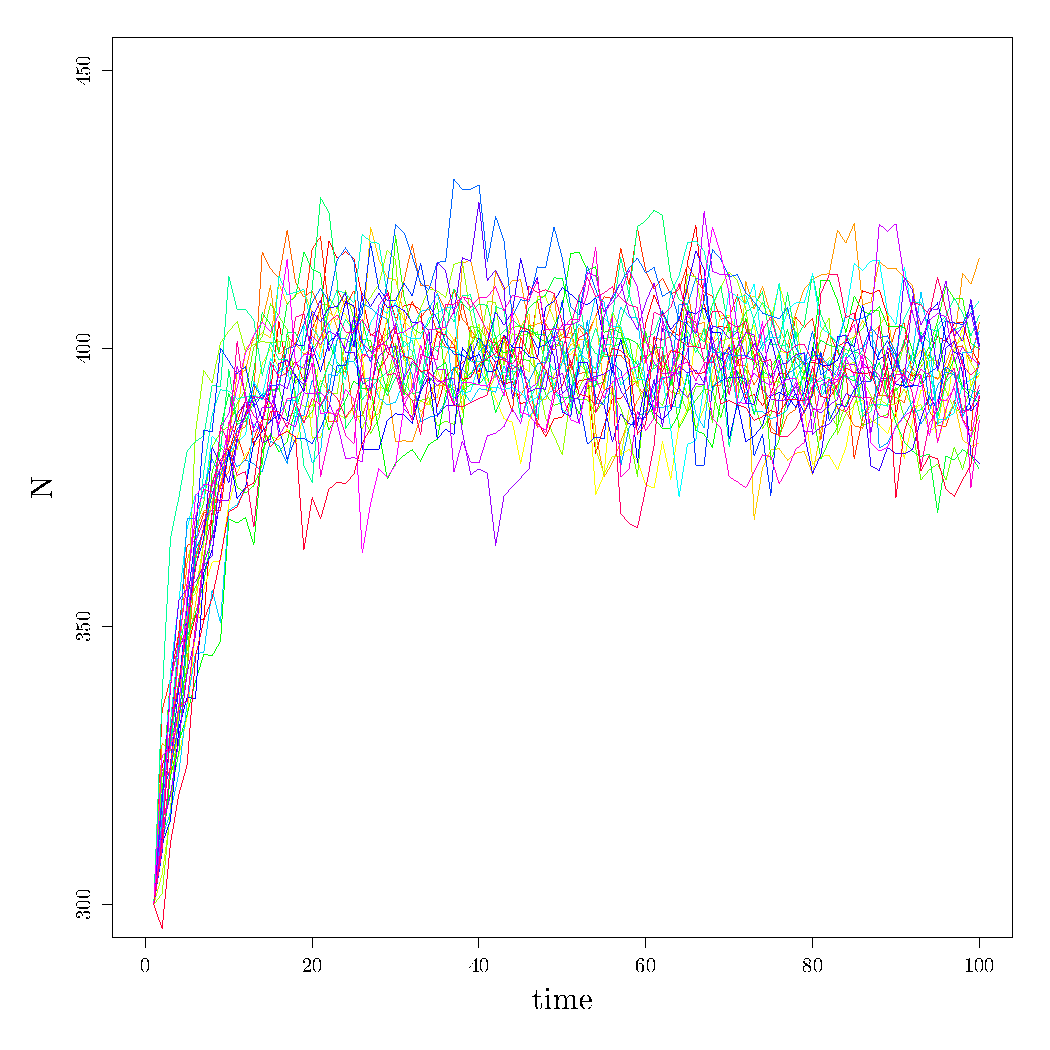
\includegraphics[width=0.65\textwidth]{figure/k22-1} 

}



\end{knitrout}
To create this plot, we need to perform the model multiple times: to do so we put it in a for-loop. This procedure is outlined below:
\begin{knitrout}
\definecolor{shadecolor}{rgb}{0.969, 0.969, 0.969}\color{fgcolor}\begin{kframe}
\begin{alltt}
\hlcom{# First we create an empty plot that will later}
\hlcom{# contain the different lines. We set the range}
\hlcom{# of the axes (xlim,ylim) and by setting type=}
\hlcom{# "n", we specify that no data should be}
\hlcom{# plotted yet.}

\hlkwd{plot}\hlstd{(}\hlnum{0}\hlstd{,}\hlnum{0}\hlstd{,}\hlkwc{xlim}\hlstd{=}\hlkwd{c}\hlstd{(}\hlnum{0}\hlstd{,}\hlnum{100}\hlstd{),}\hlkwc{ylim}\hlstd{=}\hlkwd{c}\hlstd{(}\hlnum{300}\hlstd{,}\hlnum{450}\hlstd{),}
     \hlkwc{type}\hlstd{=}\hlstr{"n"}\hlstd{,}\hlkwc{xlab}\hlstd{=}\hlstr{"time"}\hlstd{,}\hlkwc{ylab}\hlstd{=}\hlstr{"N"}\hlstd{)}

\hlcom{# We define 30 colors that we will use to plot}
\hlstd{linecols}\hlkwb{=}\hlkwd{rainbow}\hlstd{(}\hlnum{30}\hlstd{)}

\hlcom{# Now we start the loop, in this example,}
\hlcom{# we created 30 realisations of the stochastic}
\hlcom{# model:}
\hlkwa{for}\hlstd{(rep} \hlkwa{in} \hlnum{1}\hlopt{:}\hlnum{30}\hlstd{)\{}

  \hlstd{...}
  \hlstd{...}

  \hlcom{# Here you have to put your code for creating}
  \hlcom{# 1 realisation of the stochastic growth model}
  \hlcom{# (this includes a loop)}

  \hlcom{# Finally we add a line with this new realisation to}
  \hlcom{# the current plot}
  \hlkwd{lines}\hlstd{(}\hlnum{1}\hlopt{:}\hlnum{100}\hlstd{,N,}\hlkwc{col}\hlstd{=linecols[rep])}
\hlstd{\}}
\end{alltt}
\end{kframe}
\end{knitrout}
If you want you can repeat this exercise with different values for the standard deviations of $K$ and $r_d$ to see how this changes the output.

\section{Demographic Stochasticity}
We finally do a short exercise on demographic stochasticity. Assume we have a small population of $10$ bears in the Swiss Alpes. In this population the chance of survival is $p=0.6$.
\vspace{1.5ex}

\begin{center}
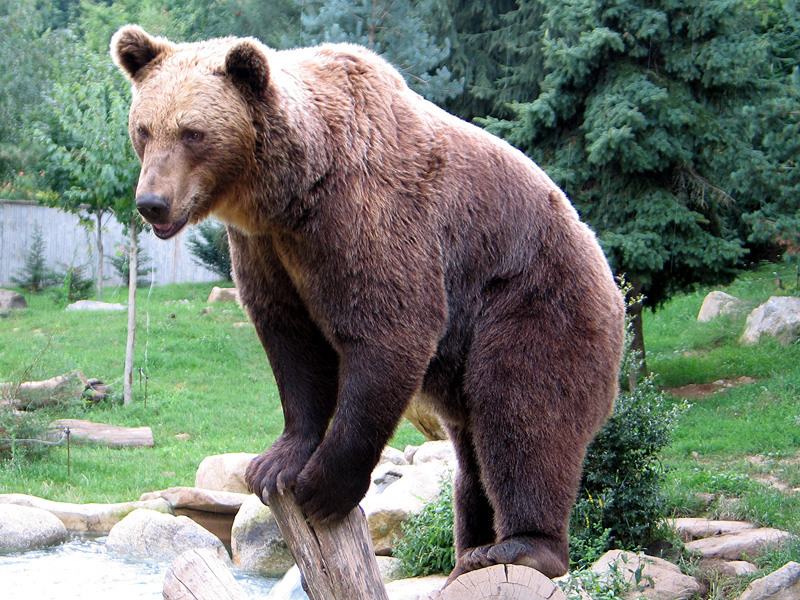
\includegraphics[width=0.65\textwidth]{Bear.jpg}
\end{center}
\vspace{1.5ex}

First we take a look at the individual. So how do we decide whether it survives or not? We draw a random number between $0$ and $1$ from a random distribution:
\begin{knitrout}
\definecolor{shadecolor}{rgb}{0.969, 0.969, 0.969}\color{fgcolor}\begin{kframe}
\begin{alltt}
\hlstd{a} \hlkwb{<-} \hlkwd{runif}\hlstd{(}\hlnum{1}\hlstd{)}
\end{alltt}
\begin{verbatim}
## 0.7186776
\end{verbatim}
\end{kframe}
\end{knitrout}
If this random number ($a$) is larger than $0.6$, the individual dies, if it is smaller than $0.6$, it survives. Because every number between $0$ and $1$ is equally likely to be drawn, this is the same thing as having a survival chance of $0.6$. In this case the individual thus dies.

We do not have $1$ individual, but we have $10$ individuals, so we need $10$ random numbers between $0$ and $1$ to determine which individuals survive:
\begin{knitrout}
\definecolor{shadecolor}{rgb}{0.969, 0.969, 0.969}\color{fgcolor}\begin{kframe}
\begin{alltt}
\hlstd{a} \hlkwb{<-} \hlkwd{runif}\hlstd{(}\hlnum{10}\hlstd{)}
\end{alltt}
\begin{verbatim}
##  [1] 0.02316389 0.90885056 0.71608529 0.23073700 0.74916228
##  [6] 0.88252136 0.67751503 0.38407123 0.79324897 0.45452743
\end{verbatim}
\begin{alltt}
\hlstd{a} \hlopt{<} \hlnum{0.6}
\end{alltt}
\begin{verbatim}
##  [1]  TRUE FALSE FALSE  TRUE FALSE FALSE FALSE  TRUE FALSE
## [10]  TRUE
\end{verbatim}
\begin{alltt}
\hlkwd{sum}\hlstd{(a} \hlopt{<} \hlnum{0.6}\hlstd{)}
\end{alltt}
\begin{verbatim}
## [1] 4
\end{verbatim}
\end{kframe}
\end{knitrout}
Here we have used that \texttt{sum(a < 0.6)} counts the number of times that \texttt{a < 0.6} contains the value \texttt{TRUE}.
The proportion of surviving individuals is thus not $0.6$, but instead:
\begin{knitrout}
\definecolor{shadecolor}{rgb}{0.969, 0.969, 0.969}\color{fgcolor}\begin{kframe}
\begin{alltt}
\hlkwd{sum}\hlstd{(a} \hlopt{<} \hlnum{0.6}\hlstd{)} \hlopt{/} \hlnum{10}
\end{alltt}
\begin{verbatim}
## [1] 0.4
\end{verbatim}
\end{kframe}
\end{knitrout}
Note that the reason for this is not that the chances of survival are different, over time, but instead that this year more individuals were unlucky and as a result of that died. Hence, this is demographic stochasticity and not environmental stochasticity.

To summarise this code, we can find the proportion of surviving individuals as follows:
\begin{knitrout}
\definecolor{shadecolor}{rgb}{0.969, 0.969, 0.969}\color{fgcolor}\begin{kframe}
\begin{alltt}
\hlkwd{sum}\hlstd{(} \hlkwd{runif}\hlstd{(}\hlnum{10}\hlstd{)} \hlopt{<} \hlnum{0.6}\hlstd{)} \hlopt{/} \hlnum{10}
\end{alltt}
\end{kframe}
\end{knitrout}
Use a for loop to repeat this calculation $1000$ times and store all the results. You can plot them using \texttt{hist}. What happens to the proportions when the number of individuals increases? (assume that the chance of survival remains constant).
\begin{knitrout}
\definecolor{shadecolor}{rgb}{0.969, 0.969, 0.969}\color{fgcolor}\begin{kframe}
\begin{alltt}
\hlstd{Np} \hlkwb{<-} \hlnum{1000}
\hlstd{outcome} \hlkwb{<-} \hlstd{...} \hlcom{# Create empty vector}
\hlkwa{for}\hlstd{(i} \hlkwa{in} \hlnum{1}\hlopt{:}\hlstd{...)\{}
  \hlstd{outcome[i]} \hlkwb{<-} \hlstd{...}
\hlstd{\}}
\hlkwd{hist}\hlstd{(outcome,} \hlkwc{xlim}\hlstd{=}\hlkwd{c}\hlstd{(}\hlnum{0}\hlstd{,}\hlnum{1}\hlstd{))}
\end{alltt}
\end{kframe}
\end{knitrout}


\section{Additional Exercise}
\textbf{This exercise is extra!\\}
In case you finish the exercises fast and don't want to go home yet: can you adapt the discrete logistic growth model to incorporate a delayed density effect? (try it first without the stochasticity, then you can include the stochasticity on $r$ and $K$.)

\section{Additional information:\\ The continuous logistic growth model}
\textbf{Extra: Logistic Growth: Solving the differential equation (for those who wish to know why the solution is the solution...)}\\
\begin{equation}
\frac{dN}{dt} = r_{max} N \left( 1-\frac{N}{K}\right).
\label{keq10}
\end{equation}
With solution:
\begin{equation}
N = \frac{K}{1+\frac{K-N_0}{N_0}e^{-r_{max}t}}.
\label{keq20}
\end{equation}
We have seen in the exercise that if you have equation \ref{keq20}, one can show that it obeys equation \ref{keq10}, but how to find equation \ref{keq20} from equation \ref{keq10}? Let us first, for simplicity set $K=1$ and $r_{max}=1$ (if you want, you can repeat the exercise without doing that):
\begin{equation}
\frac{dN}{dt} = N (1 -N).
\end{equation}
First write the equation in a way such that all terms that contain $N$ are on the left side of the equation and all terms containing $t$ on the right side:
\begin{equation}
\frac{dN}{N(1-N)} = dt
\end{equation}
Now we need to realise that in general:
\begin{equation}
\frac{1}{x} + \frac{1}{1-x} = \frac{1-x}{x(1-x)}+\frac{x}{x(1-x)} = \frac{1-x+x}{x(1-x)} = \frac{1}{x(1-x)}
\end{equation}
Using this we can write:
\begin{equation}
\frac{dN}{N} + \frac{dN}{1-N} = dt
\end{equation}
Now we take the primitive on the left and the right side of the equation:
\begin{equation}
\ln(N) + C_1 - \ln(1-N) + C_2 = t + C_3
\end{equation}
Let us group all these constants together in a new constant:
\begin{equation}
C = C_2 + C_3 - C_1
\end{equation}
Now:
\begin{equation}
\ln(N) - \ln(1-N) = t + C
\end{equation}
We take the exponential on both sides:
\begin{equation}
e^{\left(\ln(N) - \ln(1-N)\right)} = e^{t + C}
\end{equation}
Next we use that $e^{a+b} = e^a e^b$ and that $e^{-x}=\frac{1}{e^x}$:
\begin{equation}
\frac{e^{\left(\ln(N)\right)}}{e^{\left(\ln(1-N)\right)}} = e^C e^t
\end{equation}
Now we use that $e^{\ln(x)}=x$ and we define a new constant: $A=e^C$
\begin{equation}
\frac{N}{1-N} = A e^t
\end{equation}
Rewriting this equation:
\begin{equation}
N = (1-N) A e^t = A e^t - A N e^t
\end{equation}
And thus:
\begin{equation}
N (1+Ae^t) = A e^t
\end{equation}
\begin{equation}
N = \frac{Ae^t}{1+Ae^t}
\end{equation}
Now we divide the numerator and the denominator on the right side by $Ae^t$ to get the solution to the equation:
\begin{equation}
N = \frac{1}{1+\frac{1}{A}e^{-t}}
\end{equation}
Next, we know that at $t=0$, $N=N_0$, so we plug this in the equation:
\begin{equation}
N_0 = \frac{1}{1+\frac{1}{A}e^{0}} = \frac{1}{1+\frac{1}{A}}
\end{equation}
Now:
\begin{equation}
\left(1+\frac{1}{A}\right) N_0 = 1
\end{equation}
So:
\begin{equation}
1+\frac{1}{A} = \frac{1}{N_0}
\end{equation}
\begin{equation}
\frac{1}{A} = \frac{1}{N_0} -1 = \frac{1}{N_0} - \frac{N_0}{N_0} = \frac{1-N_0}{N_0} 
\end{equation}
Plugging this into the solution that we found:
\begin{equation}
N = \frac{1}{1+\frac{1-N_0}{N_0}e^{-t}}
\end{equation}

\textbf{This information is extra!\\}
\section{Answers to the \textit{pen \& paper} exercises}
\shipoutAnswer

\end{document}
